\documentclass[a4paper,11pt]{article}
\usepackage{geometry}
\geometry{top=2.5cm,bottom=2.0cm,left=1cm,right=1cm}
\usepackage{pdflscape}
\usepackage{multirow}
\usepackage{siunitx}
\usepackage{makecell}
\usepackage{xltabular}
\usepackage{amsmath}
\usepackage{booktabs}
\usepackage{authblk}
\usepackage{graphicx}
\usepackage{float}


\usepackage[dvipsnames]{xcolor}

\usepackage{fancyvrb}

% redefine \VerbatimInput
\RecustomVerbatimCommand{\VerbatimInput}{VerbatimInput}%
{fontsize=\footnotesize,
 %
 frame=lines,  % top and bottom rule only
 framesep=2em, % separation between frame and text
 rulecolor=\color{Gray},
 %
 label=\fbox{\color{Black}log.txt},
 labelposition=topline,
 %
 commandchars=\|\(\), % escape character and argument delimiters for
                      % commands within the verbatim
 commentchar=*        % comment character
}

\title{Consolidated Performance Tests}



\author[1]{Felipe Fidalgo\thanks{felipe.fidalgo@ufsc.br}}
\author[2]{Emerson Castelani\thanks{evcastelani@uem.br}}
\author[1]{Guilherme Philippi\thanks{g.philippi@grad.ufsc.br}}
\affil[1]{Department of Mathematics, Universidade Federal de Santa Catarina,
2514 João Pessoa street, Velha,
Blumenau, Santa Catarina,
Brazil,
89036-004}
\affil[2]{Department of Mathematics, Universidade Estadual de Maringá, 5790 Colombo Avenue, \\ Jardim Universitário, Maringá, Paraná, Brazil, 87020-900}

\begin{document}
	\maketitle
	\tableofcontents
	

	\newpage
	\section{Benchmark's tables}
	\subsection{Using BP-One versions}
	\begin{scriptsize}
		\begin{xltabular}{\textwidth}{r|rcS[table-format=1.4e+2]cS[table-format=1.3e+2]S[table-format=1.4e+2]S[table-format=-1.3]}
		\caption{Results} \label{tab:genResults}\\
		\toprule
		\multicolumn{1}{c}{$\begin{array}{r}
	\text{Problem}\\ \text{Size}
	\end{array}$} & Method & $|\mathcal{X}|$ & \multicolumn{1}{c}{$\begin{array}{c}
	\min\limits_{\mathbf{x}\in \mathcal{X}} \text{RMSD}(\mathbf{x},\mathbf{x}_o)
	\end{array}$} & $i : \mathbf{x_i} \sim \mathbf{x}_o$ & \multicolumn{1}{c}{$\begin{array}{c}
	\text{MDE}(\mathbf{x}_i)
	\end{array}$} & \multicolumn{1}{c}{Time} & \multicolumn{1}{c}{Improv time} \\
		\midrule
		\endfirsthead
		\caption{Results - continued}\\
		\toprule
		\multicolumn{1}{c}{$\begin{array}{r}
	\text{Problem}\\ \text{Size}
	\end{array}$} & Method & $|\mathcal{X}|$ & \multicolumn{1}{c}{$\begin{array}{c}
	\min\limits_{\mathbf{x}\in \mathcal{X}} \text{RMSD}(\mathbf{x},\mathbf{x}_o)
	\end{array}$} & $i : \mathbf{x_i} \sim \mathbf{x}_o$ & \multicolumn{1}{c}{$\begin{array}{c}
	\text{MDE}(\mathbf{x}_i)
	\end{array}$} & \multicolumn{1}{c}{Time} & \multicolumn{1}{c}{Improv time} \\
		\midrule
		\endhead
pdb1a57 & ClassicAll & 8 & 3.1806e-11 & 5 & 2.096e-11 & 7.2809e-03 & \\
698 & QuaternionAll & 8 & 3.3550e-11 & 5 & 2.092e-11 & 4.4689e-03 & 62.924\\ \cline{2-8} \addlinespace
pdb1b4c & ClassicAll & 8 & 2.6824e-12 & 5 & 5.067e-13 & 2.1270e-02 & \\
1108 & QuaternionAll & 8 & 3.4662e-12 & 5 & 5.493e-13 & 1.1014e-02 & 93.111\\ \cline{2-8} \addlinespace
pdb1ba5 & ClassicAll & 8 & 3.5621e-02 & 6 & 9.363e-13 & 2.2124e-03 & \\
320 & QuaternionAll & 8 & 3.5621e-02 & 6 & 1.069e-12 & 1.3907e-03 & 59.080\\ \cline{2-8} \addlinespace
pdb1d1n & ClassicAll & 2 & 2.9766e-11 & 1 & 1.005e-11 & 3.4032e-03 & \\
594 & QuaternionAll & 2 & 2.9311e-11 & 1 & 9.672e-12 & 1.9161e-03 & 77.609\\ \cline{2-8} \addlinespace
pdb1dp3 & ClassicAll & 8 & 4.9981e-05 & 2 & 7.704e-13 & 2.2429e-03 & \\
332 & QuaternionAll & 8 & 4.9981e-05 & 2 & 8.940e-13 & 1.4111e-03 & 58.951\\ \cline{2-8} \addlinespace
pdb1du1 & ClassicAll & 8 & 6.6600e-13 & 1 & 8.225e-13 & 7.7298e-04 & \\
122 & QuaternionAll & 8 & 1.6577e-12 & 1 & 1.258e-12 & 4.9516e-04 & 56.105\\ \cline{2-8} \addlinespace
pdb1eii & ClassicAll & 8 & 1.9451e-10 & 1 & 1.393e-11 & 5.7589e-03 & \\
806 & QuaternionAll & 8 & 1.8740e-10 & 1 & 1.365e-11 & 3.7056e-03 & 55.412\\ \cline{2-8} \addlinespace
pdb1fcl & ClassicAll & 8 & 1.5447e-11 & 2 & 4.542e-12 & 2.3324e-03 & \\
338 & QuaternionAll & 8 & 1.5223e-11 & 2 & 4.515e-12 & 1.4894e-03 & 56.596\\ \cline{2-8} \addlinespace
pdb1fd6 & ClassicAll & 8 & 2.0242e-05 & 2 & 3.182e-12 & 2.3914e-03 & \\
344 & QuaternionAll & 8 & 2.0242e-05 & 2 & 3.193e-12 & 1.5226e-03 & 57.064\\ \cline{2-8} \addlinespace
pdb1hf9 & ClassicAll & 8 & 9.0139e-10 & 6 & 1.156e-11 & 4.1332e-02 & \\
496 & QuaternionAll & 8 & 9.0282e-10 & 6 & 1.180e-11 & 2.0990e-02 & 96.917\\ \cline{2-8} \addlinespace
pdb1i2u & ClassicAll & 8 & 1.3842e-03 & 2 & 5.562e-13 & 1.8534e-03 & \\
266 & QuaternionAll & 8 & 1.3842e-03 & 2 & 5.609e-13 & 1.1875e-03 & 56.070\\ \cline{2-8} \addlinespace
pdb1i2v & ClassicAll & 8 & 8.9125e-13 & 5 & 2.422e-13 & 1.8262e-03 & \\
266 & QuaternionAll & 8 & 8.8206e-13 & 5 & 2.525e-13 & 1.1632e-03 & 56.991\\ \cline{2-8} \addlinespace
pdb1ijc & ClassicAll & 8 & 9.1858e-11 & 2 & 1.408e-11 & 2.8644e-03 & \\
380 & QuaternionAll & 8 & 9.4110e-11 & 2 & 1.426e-11 & 1.8095e-03 & 58.300\\ \cline{2-8} \addlinespace
pdb1jlz & ClassicAll & 8 & 1.2304e-04 & 1 & 5.594e-13 & 9.0730e-04 & \\
140 & QuaternionAll & 8 & 1.2304e-04 & 1 & 5.965e-13 & 5.8144e-04 & 56.042\\ \cline{2-8} \addlinespace
pdb1jw3 & ClassicAll & 8 & 1.9618e-12 & 2 & 5.936e-13 & 5.9709e-03 & \\
842 & QuaternionAll & 8 & 1.8088e-12 & 2 & 5.897e-13 & 3.8538e-03 & 54.936\\ \cline{2-8} \addlinespace
pdb1k0v & ClassicAll & 8 & 8.3940e-05 & 2 & 1.893e-13 & 3.2364e-03 & \\
440 & QuaternionAll & 8 & 8.3940e-05 & 2 & 1.894e-13 & 2.0893e-03 & 54.901\\ \cline{2-8} \addlinespace
pdb1k2h & ClassicAll & 8 & 1.9788e-04 & 2 & 5.490e-13 & 2.7044e-02 & \\
1120 & QuaternionAll & 8 & 1.9788e-04 & 2 & 5.198e-13 & 1.3022e-02 & 107.683\\ \cline{2-8} \addlinespace
pdb1k36 & ClassicAll & 8 & 1.6100e-10 & 1 & 8.820e-12 & 1.8713e-03 & \\
278 & QuaternionAll & 8 & 1.8077e-10 & 1 & 1.081e-11 & 1.1761e-03 & 59.108\\ \cline{2-8} \addlinespace
pdb1k37 & ClassicAll & 8 & 2.1407e-12 & 2 & 4.711e-13 & 1.8741e-03 & \\
278 & QuaternionAll & 8 & 2.0318e-12 & 2 & 4.988e-13 & 1.1766e-03 & 59.281\\ \cline{2-8} \addlinespace
pdb1kuw & ClassicAll & 8 & 1.8706e-04 & 1 & 9.229e-14 & 3.9350e-04 & \\
62 & QuaternionAll & 8 & 1.8706e-04 & 1 & 1.130e-13 & 2.5347e-04 & 55.244\\ \cline{2-8} \addlinespace
pdb1kz0 & ClassicAll & 8 & 6.7512e-13 & 1 & 4.404e-14 & 6.3160e-04 & \\
98 & QuaternionAll & 8 & 6.2568e-13 & 1 & 5.880e-14 & 4.0873e-04 & 54.527\\ \cline{2-8} \addlinespace
pdb1kz2 & ClassicAll & 8 & 3.1076e-06 & 1 & 2.119e-14 & 6.3818e-04 & \\
98 & QuaternionAll & 8 & 3.1076e-06 & 1 & 2.886e-14 & 4.1544e-04 & 53.617\\ \cline{2-8} \addlinespace
pdb1kz5 & ClassicAll & 8 & 4.8094e-13 & 1 & 4.081e-14 & 4.6741e-04 & \\
74 & QuaternionAll & 8 & 5.2716e-13 & 1 & 4.738e-14 & 3.0297e-04 & 54.274\\ \cline{2-8} \addlinespace
pdb1lvz & ClassicAll & 8 & 1.4708e-03 & 1 & 6.336e-14 & 4.2637e-04 & \\
68 & QuaternionAll & 8 & 1.4708e-03 & 1 & 7.315e-14 & 2.7673e-04 & 54.072\\ \cline{2-8} \addlinespace
pdb1m4e & ClassicAll & 8 & 5.4966e-12 & 1 & 5.949e-13 & 7.8262e-04 & \\
122 & QuaternionAll & 8 & 5.5048e-12 & 1 & 5.972e-13 & 5.0591e-04 & 54.695\\ \cline{2-8} \addlinespace
pdb1ma2 & ClassicAll & 8 & 1.7458e-10 & 2 & 8.695e-12 & 6.6367e-04 & \\
104 & QuaternionAll & 8 & 1.7467e-10 & 2 & 8.757e-12 & 4.2519e-04 & 56.089\\ \cline{2-8} \addlinespace
pdb1ma4 & ClassicAll & 8 & 5.4569e-04 & 2 & 7.247e-14 & 1.6300e-03 & \\
104 & QuaternionAll & 8 & 5.4569e-04 & 2 & 7.977e-14 & 9.1182e-04 & 78.766\\ \cline{2-8} \addlinespace
pdb1ma5 & ClassicAll & 8 & 9.6358e-05 & 1 & 8.169e-13 & 6.6642e-04 & \\
104 & QuaternionAll & 8 & 9.6358e-05 & 1 & 9.044e-13 & 4.2750e-04 & 55.888\\ \cline{2-8} \addlinespace
pdb1ma6 & ClassicAll & 8 & 1.2440e-11 & 2 & 6.283e-13 & 6.7054e-04 & \\
104 & QuaternionAll & 8 & 1.4288e-11 & 2 & 8.487e-13 & 4.3107e-04 & 55.552\\ \cline{2-8} \addlinespace
pdb1mpe & ClassicAll & 8 & 5.1722e-10 & 2 & 2.617e-11 & 1.2972e-02 & \\
1352 & QuaternionAll & 8 & 5.1751e-10 & 2 & 2.624e-11 & 7.0862e-03 & 83.059\\ \cline{2-8} \addlinespace
pdb1nd9 & ClassicAll & 8 & 1.0508e-12 & 2 & 3.026e-13 & 2.0665e-03 & \\
296 & QuaternionAll & 8 & 8.9082e-13 & 2 & 3.845e-13 & 1.3311e-03 & 55.244\\ \cline{2-8} \addlinespace
pdb1ne5 & ClassicAll & 128 & 1.4845e-11 & 33 & 1.214e-12 & 3.1324e-02 & \\
254 & QuaternionAll & 128 & 1.5105e-11 & 33 & 1.384e-12 & 1.9268e-02 & 62.572\\ \cline{2-8} \addlinespace
pdb1nmj & ClassicAll & 8 & 2.3883e-13 & 7 & 1.236e-14 & 1.1136e-03 & \\
170 & QuaternionAll & 8 & 2.3832e-13 & 7 & 1.422e-14 & 7.1306e-04 & 56.172\\ \cline{2-8} \addlinespace
pdb1o53 & ClassicAll & 8 & 1.0887e-11 & 2 & 3.999e-13 & 5.8436e-04 & \\
92 & QuaternionAll & 8 & 1.1252e-11 & 2 & 4.527e-13 & 3.7948e-04 & 53.989\\ \cline{2-8} \addlinespace
pdb1oqp & ClassicAll & 8 & 2.9348e-03 & 2 & 7.045e-14 & 2.6389e-02 & \\
580 & QuaternionAll & 8 & 2.9348e-03 & 2 & 8.314e-14 & 1.2611e-02 & 109.251\\ \cline{2-8} \addlinespace
pdb1plw & ClassicAll & 8 & 3.0310e-13 & 2 & 2.830e-14 & 1.8337e-04 & \\
32 & QuaternionAll & 8 & 3.2973e-13 & 2 & 3.112e-14 & 1.2031e-04 & 52.409\\ \cline{2-8} \addlinespace
pdb1plx & ClassicAll & 8 & 2.8525e-04 & 1 & 1.574e-13 & 1.8227e-04 & \\
32 & QuaternionAll & 8 & 2.8525e-04 & 1 & 2.060e-13 & 1.1973e-04 & 52.240\\ \cline{2-8} \addlinespace
pdb1pv0 & ClassicAll & 16 & 1.3024e-11 & 1 & 2.409e-13 & 3.6571e-03 & \\
278 & QuaternionAll & 16 & 1.3017e-11 & 1 & 2.723e-13 & 2.3316e-03 & 56.850\\ \cline{2-8} \addlinespace
pdb1pzr & ClassicAll & 8 & 3.9940e-10 & 1 & 5.644e-12 & 1.3561e-01 & \\
724 & QuaternionAll & 8 & 3.9046e-10 & 1 & 5.871e-12 & 6.3596e-02 & 113.244\\ \cline{2-8} \addlinespace
pdb1qlk & ClassicAll & 8 & 3.1378e-05 & 5 & 2.634e-13 & 3.4307e-02 & \\
1108 & QuaternionAll & 8 & 3.1378e-05 & 5 & 2.870e-13 & 1.8207e-02 & 88.432\\ \cline{2-8} \addlinespace
pdb1r57 & ClassicAll & 8 & 4.3330e-03 & 2 & 1.847e-13 & 4.3256e-03 & \\
614 & QuaternionAll & 8 & 4.3330e-03 & 2 & 2.054e-13 & 2.7794e-03 & 55.629\\ \cline{2-8} \addlinespace
pdb1ry3 & ClassicAll & 8 & 9.1924e-12 & 2 & 4.938e-13 & 2.6869e-03 & \\
386 & QuaternionAll & 8 & 9.4285e-12 & 2 & 5.913e-13 & 1.6911e-03 & 58.887\\ \cline{2-8} \addlinespace
pdb1s4h & ClassicAll & 8 & 1.4643e-04 & 2 & 4.696e-13 & 5.0092e-04 & \\
80 & QuaternionAll & 8 & 1.4643e-04 & 2 & 6.351e-13 & 3.2082e-04 & 56.137\\ \cline{2-8} \addlinespace
pdb1s4j & ClassicAll & 8 & 5.8507e-12 & 2 & 1.520e-13 & 5.0893e-04 & \\
80 & QuaternionAll & 8 & 5.8479e-12 & 2 & 2.083e-13 & 3.2814e-04 & 55.098\\ \cline{2-8} \addlinespace
pdb1s6j & ClassicAll & 8 & 6.0202e-05 & 1 & 6.073e-13 & 3.6427e-03 & \\
524 & QuaternionAll & 8 & 6.0202e-05 & 1 & 7.660e-13 & 2.3187e-03 & 57.105\\ \cline{2-8} \addlinespace
pdb1sa8 & ClassicAll & 8 & 1.7170e-03 & 1 & 9.340e-13 & 4.5237e-03 & \\
638 & QuaternionAll & 8 & 1.7170e-03 & 1 & 1.034e-12 & 2.9180e-03 & 55.028\\ \cline{2-8} \addlinespace
pdb1t2y & ClassicAll & 8 & 2.5460e-04 & 1 & 1.887e-13 & 1.0049e-03 & \\
152 & QuaternionAll & 8 & 2.5460e-04 & 1 & 2.396e-13 & 6.4634e-04 & 55.471\\ \cline{2-8} \addlinespace
pdb1t5q & ClassicAll & 2 & 1.0265e-12 & 1 & 3.877e-14 & 9.4140e-04 & \\
180 & QuaternionAll & 2 & 1.0480e-12 & 1 & 5.093e-14 & 5.2229e-04 & 80.246\\ \cline{2-8} \addlinespace
pdb1tot & ClassicAll & 8 & 3.4218e-03 & 5 & 6.151e-14 & 2.2248e-03 & \\
314 & QuaternionAll & 8 & 3.4218e-03 & 5 & 6.855e-14 & 1.4150e-03 & 57.226\\ \cline{2-8} \addlinespace
pdb1v6r & ClassicAll & 8 & 1.3650e-04 & 2 & 6.835e-13 & 8.2326e-04 & \\
128 & QuaternionAll & 8 & 1.3650e-04 & 2 & 6.971e-13 & 5.3413e-04 & 54.130\\ \cline{2-8} \addlinespace
pdb1v92 & ClassicAll & 8 & 3.1327e-05 & 1 & 1.463e-13 & 1.9147e-03 & \\
278 & QuaternionAll & 8 & 3.1327e-05 & 1 & 1.630e-13 & 1.2218e-03 & 56.713\\ \cline{2-8} \addlinespace
pdb1vd7 & ClassicAll & 8 & 7.8801e-12 & 1 & 6.342e-13 & 8.9838e-04 & \\
140 & QuaternionAll & 8 & 7.9022e-12 & 1 & 7.439e-13 & 5.7692e-04 & 55.722\\ \cline{2-8} \addlinespace
pdb1vd9 & ClassicAll & 8 & 1.5514e-11 & 1 & 1.290e-12 & 9.0145e-04 & \\
140 & QuaternionAll & 8 & 1.5541e-11 & 1 & 1.554e-12 & 5.8017e-04 & 55.375\\ \cline{2-8} \addlinespace
pdb1vdb & ClassicAll & 8 & 8.5740e-12 & 2 & 9.108e-13 & 8.9940e-04 & \\
140 & QuaternionAll & 8 & 8.5291e-12 & 2 & 1.082e-12 & 5.7863e-04 & 55.436\\ \cline{2-8} \addlinespace
pdb1vpc & ClassicAll & 8 & 4.3482e-04 & 6 & 8.510e-15 & 1.8814e-03 & \\
272 & QuaternionAll & 8 & 4.3482e-04 & 6 & 1.002e-14 & 1.1821e-03 & 59.168\\ \cline{2-8} \addlinespace
pdb1wnk & ClassicAll & 8 & 2.2292e-10 & 1 & 4.112e-12 & 9.0328e-04 & \\
140 & QuaternionAll & 8 & 2.2177e-10 & 1 & 4.632e-12 & 5.8154e-04 & 55.326\\ \cline{2-8} \addlinespace
pdb1wo4 & ClassicAll & 8 & 4.6193e-05 & 2 & 9.957e-13 & 9.8278e-04 & \\
152 & QuaternionAll & 8 & 4.6193e-05 & 2 & 9.634e-13 & 6.2760e-04 & 56.594\\ \cline{2-8} \addlinespace
pdb1wo5 & ClassicAll & 8 & 2.7147e-10 & 1 & 2.372e-12 & 9.9679e-04 & \\
152 & QuaternionAll & 8 & 2.7625e-10 & 1 & 2.514e-12 & 6.3801e-04 & 56.234\\ \cline{2-8} \addlinespace
pdb1x60 & ClassicAll & 8 & 6.7449e-12 & 1 & 1.076e-12 & 3.3185e-03 & \\
476 & QuaternionAll & 8 & 6.9447e-12 & 1 & 1.179e-12 & 2.1300e-03 & 55.794\\ \cline{2-8} \addlinespace
pdb1x9v & ClassicAll & 8 & 1.1547e-04 & 6 & 8.968e-13 & 4.1532e-02 & \\
544 & QuaternionAll & 8 & 1.1547e-04 & 6 & 9.611e-13 & 2.1462e-02 & 93.514\\ \cline{2-8} \addlinespace
pdb1y5c & ClassicAll & 8 & 8.7435e-13 & 1 & 7.693e-14 & 4.1815e-04 & \\
68 & QuaternionAll & 8 & 8.2242e-13 & 1 & 9.383e-14 & 2.6862e-04 & 55.664\\ \cline{2-8} \addlinespace
pdb1yx7 & ClassicAll & 8 & 1.3647e-10 & 5 & 3.509e-12 & 3.4921e-03 & \\
500 & QuaternionAll & 8 & 1.4245e-10 & 5 & 4.348e-12 & 2.2405e-03 & 55.859\\ \cline{2-8} \addlinespace
pdb1yx8 & ClassicAll & 8 & 2.5841e-10 & 6 & 7.284e-12 & 3.9503e-03 & \\
500 & QuaternionAll & 8 & 2.6921e-10 & 6 & 8.217e-12 & 2.4721e-03 & 59.794\\ \cline{2-8} \addlinespace
pdb1yxr & ClassicAll & 8 & 9.3459e-04 & 1 & 6.979e-13 & 3.2221e-03 & \\
464 & QuaternionAll & 8 & 9.3459e-04 & 1 & 7.989e-13 & 2.0651e-03 & 56.027\\ \cline{2-8} \addlinespace
pdb2a2y & ClassicAll & 8 & 8.1076e-05 & 2 & 1.150e-12 & 2.0742e-01 & \\
1072 & QuaternionAll & 8 & 8.1076e-05 & 2 & 1.151e-12 & 9.6631e-02 & 114.651\\ \cline{2-8} \addlinespace
pdb2a4j & ClassicAll & 8 & 1.0516e-04 & 2 & 2.085e-14 & 4.7209e-03 & \\
580 & QuaternionAll & 8 & 1.0516e-04 & 2 & 2.727e-14 & 2.9282e-03 & 61.221\\ \cline{2-8} \addlinespace
pdb2adl & ClassicAll & 8 & 3.1161e-11 & 1 & 1.752e-11 & 1.6224e-02 & \\
868 & QuaternionAll & 8 & 3.3255e-11 & 1 & 1.787e-11 & 8.2860e-03 & 95.796\\ \cline{2-8} \addlinespace
pdb2adn & ClassicAll & 8 & 2.3364e-10 & 1 & 6.693e-12 & 1.2092e-02 & \\
868 & QuaternionAll & 8 & 2.3188e-10 & 1 & 6.465e-12 & 6.2165e-03 & 94.518\\ \cline{2-8} \addlinespace
pdb2ajj & ClassicAll & 8 & 2.9810e-04 & 1 & 5.641e-14 & 1.1142e-03 & \\
170 & QuaternionAll & 8 & 2.9810e-04 & 1 & 6.584e-14 & 7.1685e-04 & 55.426\\ \cline{2-8} \addlinespace
pdb2ajm & ClassicAll & 8 & 2.4063e-12 & 2 & 1.183e-13 & 1.1178e-03 & \\
170 & QuaternionAll & 8 & 2.7001e-12 & 2 & 1.555e-13 & 7.1704e-04 & 55.888\\ \cline{2-8} \addlinespace
pdb2ajn & ClassicAll & 8 & 4.3268e-04 & 1 & 1.076e-13 & 1.1127e-03 & \\
170 & QuaternionAll & 8 & 4.3268e-04 & 1 & 1.217e-13 & 7.0951e-04 & 56.819\\ \cline{2-8} \addlinespace
pdb2ajo & ClassicAll & 8 & 2.4063e-12 & 2 & 1.183e-13 & 1.1319e-03 & \\
170 & QuaternionAll & 8 & 2.7001e-12 & 2 & 1.555e-13 & 7.2495e-04 & 56.141\\ \cline{2-8} \addlinespace
pdb2akk & ClassicAll & 8 & 3.0416e-03 & 2 & 1.289e-13 & 3.1222e-03 & \\
446 & QuaternionAll & 8 & 3.0416e-03 & 2 & 1.279e-13 & 2.0200e-03 & 54.563\\ \cline{2-8} \addlinespace
pdb2bzb & ClassicAll & 8 & 4.6498e-13 & 5 & 9.361e-14 & 4.3562e-02 & \\
748 & QuaternionAll & 8 & 6.0113e-13 & 5 & 1.224e-13 & 2.2532e-02 & 93.330\\ \cline{2-8} \addlinespace
pdb2c0s & ClassicAll & 8 & 1.0793e-02 & 6 & 3.028e-13 & 2.7457e-03 & \\
386 & QuaternionAll & 8 & 1.0793e-02 & 6 & 3.380e-13 & 1.7354e-03 & 58.218\\ \cline{2-8} \addlinespace
pdb2dci & ClassicAll & 2 & 2.0907e-13 & 1 & 2.366e-14 & 6.2917e-04 & \\
120 & QuaternionAll & 2 & 3.3732e-13 & 1 & 2.950e-14 & 3.5153e-04 & 78.979\\ \cline{2-8} \addlinespace
pdb2eem & ClassicAll & 8 & 9.5324e-12 & 1 & 5.190e-13 & 1.3791e-03 & \\
206 & QuaternionAll & 8 & 9.5866e-12 & 1 & 5.461e-13 & 8.7569e-04 & 57.484\\ \cline{2-8} \addlinespace
pdb2fva & ClassicAll & 8 & 1.2680e-11 & 2 & 1.047e-12 & 3.4456e-03 & \\
494 & QuaternionAll & 8 & 1.2689e-11 & 2 & 1.195e-12 & 2.1859e-03 & 57.630\\ \cline{2-8} \addlinespace
pdb2fvf & ClassicAll & 8 & 3.5796e-12 & 1 & 3.106e-13 & 3.4168e-03 & \\
494 & QuaternionAll & 8 & 3.3286e-12 & 1 & 3.445e-13 & 2.1795e-03 & 56.772\\ \cline{2-8} \addlinespace
pdb2fxz & ClassicAll & 8 & 4.2293e-12 & 1 & 1.489e-12 & 5.1193e-04 & \\
80 & QuaternionAll & 8 & 5.3169e-12 & 1 & 1.749e-12 & 3.3308e-04 & 53.694\\ \cline{2-8} \addlinespace
pdb2g9j & ClassicAll & 8 & 5.8011e-04 & 2 & 3.282e-12 & 2.5868e-01 & \\
848 & QuaternionAll & 8 & 5.8011e-04 & 2 & 3.535e-12 & 1.2410e-01 & 108.442\\ \cline{2-8} \addlinespace
pdb2g9l & ClassicAll & 8 & 1.0333e-04 & 2 & 6.365e-14 & 1.5218e-03 & \\
224 & QuaternionAll & 8 & 1.0333e-04 & 2 & 8.666e-14 & 9.7592e-04 & 55.930\\ \cline{2-8} \addlinespace
pdb2h5m & ClassicAll & 8 & 1.2267e-03 & 1 & 9.692e-13 & 4.3204e-03 & \\
614 & QuaternionAll & 8 & 1.2267e-03 & 1 & 1.032e-12 & 2.7745e-03 & 55.719\\ \cline{2-8} \addlinespace
pdb2hep & ClassicAll & 2 & 2.1758e-11 & 1 & 1.191e-12 & 1.3630e-03 & \\
252 & QuaternionAll & 2 & 2.2038e-11 & 1 & 1.268e-12 & 7.4289e-04 & 83.470\\ \cline{2-8} \addlinespace
pdb2j0z & ClassicAll & 8 & 1.3100e-10 & 6 & 4.392e-12 & 1.6225e-01 & \\
752 & QuaternionAll & 8 & 1.3116e-10 & 6 & 4.954e-12 & 7.6455e-02 & 112.221\\ \cline{2-8} \addlinespace
pdb2j10 & ClassicAll & 1024 & 2.9952e-05 & 574 & 9.196e-12 & 6.9076e-01 & \\
752 & QuaternionAll & 1024 & 2.9952e-05 & 574 & 9.529e-12 & 5.5744e-01 & 23.916\\ \cline{2-8} \addlinespace
pdb2j11 & ClassicAll & 1024 & 2.7803e-11 & 549 & 5.256e-12 & 6.8396e-01 & \\
752 & QuaternionAll & 1024 & 2.7661e-11 & 549 & 5.631e-12 & 5.5403e-01 & 23.451\\ \cline{2-8} \addlinespace
pdb2jmy & ClassicAll & 8 & 7.0432e-05 & 1 & 9.834e-13 & 5.9753e-04 & \\
92 & QuaternionAll & 8 & 7.0432e-05 & 1 & 9.967e-13 & 3.9079e-04 & 52.902\\ \cline{2-8} \addlinespace
pdb2jn5 & ClassicAll & 8 & 6.6339e-12 & 1 & 1.104e-11 & 4.5917e-04 & \\
74 & QuaternionAll & 8 & 2.0459e-11 & 1 & 2.456e-11 & 2.9467e-04 & 55.821\\ \cline{2-8} \addlinespace
pdb2jnk & ClassicAll & 8 & 3.4995e-11 & 1 & 2.246e-12 & 6.1289e-03 & \\
842 & QuaternionAll & 8 & 3.4653e-11 & 1 & 2.319e-12 & 3.9634e-03 & 54.638\\ \cline{2-8} \addlinespace
pdb2jpn & ClassicAll & 8 & 6.4192e-12 & 2 & 6.730e-14 & 4.4889e-03 & \\
476 & QuaternionAll & 8 & 6.5904e-12 & 2 & 6.984e-14 & 2.6999e-03 & 66.263\\ \cline{2-8} \addlinespace
pdb2jua & ClassicAll & 8 & 1.8734e-04 & 2 & 1.740e-11 & 4.4058e-03 & \\
614 & QuaternionAll & 8 & 1.8734e-04 & 2 & 1.882e-11 & 2.8125e-03 & 56.651\\ \cline{2-8} \addlinespace
pdb2jvd & ClassicAll & 2 & 9.4244e-13 & 1 & 3.339e-14 & 1.5937e-03 & \\
288 & QuaternionAll & 2 & 9.4967e-13 & 1 & 3.898e-14 & 8.6556e-04 & 84.120\\ \cline{2-8} \addlinespace
pdb2jwe & ClassicAll & 2 & 9.2597e-11 & 1 & 2.695e-11 & 5.7062e-03 & \\
984 & QuaternionAll & 2 & 9.2052e-11 & 1 & 2.734e-11 & 3.2068e-03 & 77.939\\ \cline{2-8} \addlinespace
pdb2jws & ClassicAll & 8 & 4.5612e-04 & 2 & 1.251e-13 & 2.4097e-03 & \\
338 & QuaternionAll & 8 & 4.5612e-04 & 2 & 1.543e-13 & 1.5261e-03 & 57.901\\ \cline{2-8} \addlinespace
pdb2jwu & ClassicAll & 8 & 3.0876e-04 & 1 & 4.421e-12 & 2.3772e-03 & \\
338 & QuaternionAll & 8 & 3.0876e-04 & 1 & 4.373e-12 & 1.5088e-03 & 57.553\\ \cline{2-8} \addlinespace
pdb2jxf & ClassicAll & 8 & 2.4000e-04 & 1 & 1.399e-13 & 1.2135e-03 & \\
182 & QuaternionAll & 8 & 2.4000e-04 & 1 & 1.734e-13 & 7.7392e-04 & 56.804\\ \cline{2-8} \addlinespace
pdb2jz5 & ClassicAll & 8 & 1.7460e-03 & 1 & 2.860e-13 & 3.7883e-03 & \\
548 & QuaternionAll & 8 & 1.7460e-03 & 1 & 2.854e-13 & 2.3977e-03 & 57.995\\ \cline{2-8} \addlinespace
pdb2k2a & ClassicAll & 8 & 4.7195e-03 & 5 & 3.810e-14 & 3.0023e-03 & \\
422 & QuaternionAll & 8 & 4.7195e-03 & 5 & 5.148e-14 & 1.8981e-03 & 58.171\\ \cline{2-8} \addlinespace
pdb2k36 & ClassicAll & 8 & 1.6972e-12 & 1 & 1.922e-13 & 6.4120e-03 & \\
896 & QuaternionAll & 8 & 1.6007e-12 & 1 & 2.045e-13 & 4.0937e-03 & 56.632\\ \cline{2-8} \addlinespace
pdb2k37 & ClassicAll & 8 & 3.7147e-12 & 1 & 1.921e-13 & 2.5156e-03 & \\
356 & QuaternionAll & 8 & 3.6185e-12 & 1 & 2.525e-13 & 1.6076e-03 & 56.483\\ \cline{2-8} \addlinespace
pdb2k3i & ClassicAll & 8 & 4.6225e-03 & 2 & 3.810e-13 & 5.9655e-03 & \\
656 & QuaternionAll & 8 & 4.6225e-03 & 2 & 4.009e-13 & 3.6009e-03 & 65.669\\ \cline{2-8} \addlinespace
pdb2k6s & ClassicAll & 8 & 8.2998e-12 & 2 & 2.100e-13 & 7.4448e-03 & \\
494 & QuaternionAll & 8 & 8.4519e-12 & 2 & 2.651e-13 & 4.1977e-03 & 77.352\\ \cline{2-8} \addlinespace
pdb2k7o & ClassicAll & 8 & 1.8663e-04 & 1 & 1.279e-13 & 5.1042e-02 & \\
1096 & QuaternionAll & 8 & 1.8663e-04 & 1 & 1.416e-13 & 2.6472e-02 & 92.816\\ \cline{2-8} \addlinespace
pdb2kdh & ClassicAll & 8 & 7.2209e-05 & 2 & 1.947e-11 & 3.1157e-03 & \\
434 & QuaternionAll & 8 & 7.2209e-05 & 2 & 2.228e-11 & 1.9604e-03 & 58.926\\ \cline{2-8} \addlinespace
pdb2kdl & ClassicAll & 8 & 4.4591e-12 & 2 & 2.301e-13 & 2.3420e-03 & \\
338 & QuaternionAll & 8 & 4.4513e-12 & 2 & 2.919e-13 & 1.4780e-03 & 58.453\\ \cline{2-8} \addlinespace
pdb2kdm & ClassicAll & 8 & 2.1896e-11 & 1 & 3.191e-12 & 2.3526e-03 & \\
338 & QuaternionAll & 8 & 2.1643e-11 & 1 & 3.284e-12 & 1.4931e-03 & 57.563\\ \cline{2-8} \addlinespace
pdb2kdp & ClassicAll & 8 & 3.0283e-12 & 1 & 2.621e-13 & 3.0201e-03 & \\
428 & QuaternionAll & 8 & 3.0741e-12 & 1 & 2.865e-13 & 1.9141e-03 & 57.784\\ \cline{2-8} \addlinespace
pdb2kdr & ClassicAll & 8 & 6.3024e-05 & 2 & 6.618e-14 & 1.1144e-03 & \\
170 & QuaternionAll & 8 & 6.3024e-05 & 2 & 8.490e-14 & 7.1578e-04 & 55.689\\ \cline{2-8} \addlinespace
pdb2kes & ClassicAll & 8 & 1.8528e-04 & 7 & 4.467e-14 & 1.9764e-03 & \\
290 & QuaternionAll & 8 & 1.8528e-04 & 7 & 5.425e-14 & 1.2653e-03 & 56.198\\ \cline{2-8} \addlinespace
pdb2kib & ClassicAll & 8 & 2.9706e-05 & 1 & 2.533e-12 & 3.6121e-02 & \\
352 & QuaternionAll & 8 & 2.9706e-05 & 1 & 2.539e-12 & 1.7593e-02 & 105.320\\ \cline{2-8} \addlinespace
pdb2kjn & ClassicAll & 8 & 1.9764e-12 & 2 & 9.827e-14 & 1.0238e-03 & \\
158 & QuaternionAll & 8 & 1.9265e-12 & 2 & 1.174e-13 & 6.5720e-04 & 55.786\\ \cline{2-8} \addlinespace
pdb2kjo & ClassicAll & 8 & 1.2876e-11 & 1 & 2.284e-13 & 1.0281e-03 & \\
158 & QuaternionAll & 8 & 1.2921e-11 & 1 & 2.421e-13 & 6.5279e-04 & 57.491\\ \cline{2-8} \addlinespace
pdb2kjr & ClassicAll & 8 & 5.1341e-11 & 2 & 3.247e-12 & 3.9329e-03 & \\
572 & QuaternionAll & 8 & 5.1082e-11 & 2 & 3.252e-12 & 2.4975e-03 & 57.478\\ \cline{2-8} \addlinespace
pdb2kko & ClassicAll & 8 & 6.9643e-04 & 2 & 1.191e-13 & 5.7594e-02 & \\
1300 & QuaternionAll & 8 & 6.9643e-04 & 2 & 1.284e-13 & 2.9551e-02 & 94.893\\ \cline{2-8} \addlinespace
pdb2kl5 & ClassicAll & 8 & 2.4505e-12 & 1 & 1.820e-13 & 4.6396e-03 & \\
662 & QuaternionAll & 8 & 2.5206e-12 & 1 & 2.020e-13 & 2.9536e-03 & 57.082\\ \cline{2-8} \addlinespace
pdb2klz & ClassicAll & 2 & 3.9786e-13 & 1 & 3.439e-14 & 1.5092e-03 & \\
276 & QuaternionAll & 2 & 3.7834e-13 & 1 & 4.443e-14 & 8.1938e-04 & 84.188\\ \cline{2-8} \addlinespace
pdb2ko1 & ClassicAll & 8 & 9.3273e-04 & 2 & 1.150e-12 & 8.1846e-02 & \\
1060 & QuaternionAll & 8 & 9.3273e-04 & 2 & 1.151e-12 & 3.8900e-02 & 110.404\\ \cline{2-8} \addlinespace
pdb2koz & ClassicAll & 8 & 4.7204e-05 & 2 & 1.067e-12 & 1.3779e-03 & \\
200 & QuaternionAll & 8 & 4.7204e-05 & 2 & 1.151e-12 & 8.9375e-04 & 54.175\\ \cline{2-8} \addlinespace
pdb2kp0 & ClassicAll & 8 & 7.8392e-11 & 2 & 4.894e-12 & 1.3406e-03 & \\
200 & QuaternionAll & 8 & 8.2404e-11 & 2 & 5.595e-12 & 8.5529e-04 & 56.740\\ \cline{2-8} \addlinespace
pdb2ksg & ClassicAll & 8 & 9.2027e-13 & 1 & 3.215e-14 & 1.9736e-03 & \\
290 & QuaternionAll & 8 & 9.2208e-13 & 1 & 3.967e-14 & 1.2418e-03 & 58.929\\ \cline{2-8} \addlinespace
pdb2kt8 & ClassicAll & 8 & 4.1573e-04 & 1 & 3.314e-12 & 3.1511e-03 & \\
458 & QuaternionAll & 8 & 4.1573e-04 & 1 & 3.535e-12 & 1.9983e-03 & 57.688\\ \cline{2-8} \addlinespace
pdb2kuh & ClassicAll & 8 & 1.1667e-03 & 6 & 2.015e-14 & 2.8587e-03 & \\
404 & QuaternionAll & 8 & 1.1667e-03 & 6 & 2.491e-14 & 1.8319e-03 & 56.056\\ \cline{2-8} \addlinespace
pdb2kwh & ClassicAll & 8 & 2.0587e-03 & 2 & 1.408e-13 & 2.3533e-03 & \\
338 & QuaternionAll & 8 & 2.0587e-03 & 2 & 1.825e-13 & 1.4928e-03 & 57.645\\ \cline{2-8} \addlinespace
pdb2kxa & ClassicAll & 2 & 3.9712e-12 & 1 & 1.325e-12 & 7.7669e-04 & \\
144 & QuaternionAll & 2 & 3.7392e-12 & 1 & 1.351e-12 & 4.3576e-04 & 78.240\\ \cline{2-8} \addlinespace
pdb2kyb & ClassicAll & 8 & 3.1200e-06 & 2 & 1.321e-11 & 3.3785e-03 & \\
362 & QuaternionAll & 8 & 3.1200e-06 & 2 & 1.373e-11 & 2.0218e-03 & 67.103\\ \cline{2-8} \addlinespace
pdb2l3m & ClassicAll & 8 & 1.5178e-03 & 1 & 1.028e-12 & 2.9880e-03 & \\
428 & QuaternionAll & 8 & 1.5178e-03 & 1 & 9.340e-13 & 1.9052e-03 & 56.832\\ \cline{2-8} \addlinespace
pdb2l3n & ClassicAll & 8 & 3.9987e-04 & 5 & 3.024e-14 & 1.8292e-02 & \\
626 & QuaternionAll & 8 & 3.9987e-04 & 5 & 3.632e-14 & 9.1060e-03 & 100.878\\ \cline{2-8} \addlinespace
pdb2l45 & ClassicAll & 8 & 5.9466e-13 & 1 & 2.236e-14 & 7.4857e-04 & \\
116 & QuaternionAll & 8 & 6.7808e-13 & 1 & 3.033e-14 & 4.8326e-04 & 54.902\\ \cline{2-8} \addlinespace
pdb2l5r & ClassicAll & 2 & 3.0491e-13 & 2 & 3.535e-14 & 7.1313e-04 & \\
138 & QuaternionAll & 2 & 3.0031e-13 & 2 & 4.436e-14 & 3.9530e-04 & 80.404\\ \cline{2-8} \addlinespace
pdb2l6q & ClassicAll & 4 & 1.6115e-09 & 1 & 4.435e-11 & 1.9702e-03 & \\
374 & QuaternionAll & 4 & 1.6752e-09 & 1 & 5.413e-11 & 1.1676e-03 & 68.740\\ \cline{2-8} \addlinespace
pdb2l6r & ClassicAll & 8 & 1.0970e-10 & 2 & 2.060e-12 & 2.6126e-03 & \\
374 & QuaternionAll & 8 & 9.8250e-11 & 2 & 2.174e-12 & 1.6511e-03 & 58.241\\ \cline{2-8} \addlinespace
pdb2l98 & ClassicAll & 8 & 5.6413e-12 & 2 & 3.273e-13 & 2.9948e-03 & \\
434 & QuaternionAll & 8 & 6.2089e-12 & 2 & 3.637e-13 & 1.9033e-03 & 57.346\\ \cline{2-8} \addlinespace
pdb2lci & ClassicAll & 8 & 1.2015e-12 & 1 & 2.579e-13 & 5.7213e-03 & \\
806 & QuaternionAll & 8 & 1.1830e-12 & 1 & 2.404e-13 & 3.6569e-03 & 56.453\\ \cline{2-8} \addlinespace
pdb2lde & ClassicAll & 8 & 6.0406e-03 & 2 & 3.154e-14 & 9.7258e-04 & \\
152 & QuaternionAll & 8 & 6.0406e-03 & 2 & 3.766e-14 & 6.2382e-04 & 55.908\\ \cline{2-8} \addlinespace
pdb2le2 & ClassicAll & 8 & 1.5317e-12 & 2 & 2.064e-13 & 2.2550e-01 & \\
676 & QuaternionAll & 8 & 1.4989e-12 & 2 & 2.042e-13 & 1.0775e-01 & 109.289\\ \cline{2-8} \addlinespace
pdb2le7 & ClassicAll & 8 & 8.8940e-14 & 2 & 2.111e-14 & 7.8628e-04 & \\
122 & QuaternionAll & 8 & 1.1008e-13 & 2 & 2.749e-14 & 5.0699e-04 & 55.086\\ \cline{2-8} \addlinespace
pdb2ler & ClassicAll & 8 & 5.1096e-14 & 2 & 1.314e-14 & 4.2219e-04 & \\
68 & QuaternionAll & 8 & 6.2001e-14 & 2 & 1.532e-14 & 2.7220e-04 & 55.103\\ \cline{2-8} \addlinespace
pdb2lgi & ClassicAll & 8 & 9.7255e-12 & 2 & 1.068e-12 & 2.3777e-03 & \\
338 & QuaternionAll & 8 & 9.6518e-12 & 2 & 1.052e-12 & 1.5290e-03 & 55.512\\ \cline{2-8} \addlinespace
pdb2lhc & ClassicAll & 8 & 3.8367e-10 & 1 & 2.902e-12 & 2.4530e-03 & \\
338 & QuaternionAll & 8 & 3.8166e-10 & 1 & 2.997e-12 & 1.5355e-03 & 59.753\\ \cline{2-8} \addlinespace
pdb2lhd & ClassicAll & 8 & 1.3048e-11 & 2 & 1.930e-12 & 2.3310e-03 & \\
338 & QuaternionAll & 8 & 1.4592e-11 & 2 & 2.033e-12 & 1.4876e-03 & 56.692\\ \cline{2-8} \addlinespace
pdb2lhe & ClassicAll & 8 & 9.7862e-10 & 2 & 4.963e-11 & 2.5778e-03 & \\
338 & QuaternionAll & 8 & 9.7867e-10 & 2 & 4.967e-11 & 1.6222e-03 & 58.911\\ \cline{2-8} \addlinespace
pdb2lhg & ClassicAll & 8 & 5.0995e-13 & 6 & 6.485e-14 & 2.3574e-03 & \\
338 & QuaternionAll & 8 & 5.4683e-13 & 6 & 7.343e-14 & 1.5033e-03 & 56.813\\ \cline{2-8} \addlinespace
pdb2lix & ClassicAll & 2 & 4.9988e-13 & 1 & 4.842e-14 & 8.5820e-04 & \\
162 & QuaternionAll & 2 & 5.1517e-13 & 1 & 5.614e-14 & 4.8147e-04 & 78.248\\ \cline{2-8} \addlinespace
pdb2lld & ClassicAll & 8 & 3.3972e-03 & 5 & 1.938e-13 & 1.6475e-03 & \\
242 & QuaternionAll & 8 & 3.3972e-03 & 5 & 2.216e-13 & 1.0545e-03 & 56.234\\ \cline{2-8} \addlinespace
pdb2lm9 & ClassicAll & 8 & 2.2967e-03 & 2 & 6.254e-14 & 4.0327e-03 & \\
578 & QuaternionAll & 8 & 2.2967e-03 & 2 & 7.713e-14 & 2.5610e-03 & 57.467\\ \cline{2-8} \addlinespace
pdb2lmf & ClassicAll & 8 & 1.0942e-04 & 1 & 1.282e-13 & 9.0512e-04 & \\
140 & QuaternionAll & 8 & 1.0942e-04 & 1 & 1.462e-13 & 5.8774e-04 & 53.999\\ \cline{2-8} \addlinespace
pdb2ln3 & ClassicAll & 8 & 2.5821e-13 & 1 & 1.292e-13 & 3.4721e-03 & \\
500 & QuaternionAll & 8 & 2.9987e-13 & 1 & 1.359e-13 & 2.2061e-03 & 57.389\\ \cline{2-8} \addlinespace
pdb2lo2 & ClassicAll & 8 & 1.4423e-02 & 2 & 2.068e-14 & 1.5554e-03 & \\
230 & QuaternionAll & 8 & 1.4423e-02 & 2 & 2.571e-14 & 9.9098e-04 & 56.953\\ \cline{2-8} \addlinespace
pdb2lqp & ClassicAll & 8 & 5.7815e-04 & 2 & 2.950e-13 & 2.9979e-03 & \\
428 & QuaternionAll & 8 & 5.7815e-04 & 2 & 3.085e-13 & 1.9145e-03 & 56.593\\ \cline{2-8} \addlinespace
pdb2lr0 & ClassicAll & 8 & 1.2202e-11 & 1 & 3.549e-12 & 5.7308e-03 & \\
806 & QuaternionAll & 8 & 1.1747e-11 & 1 & 3.440e-12 & 3.6589e-03 & 56.626\\ \cline{2-8} \addlinespace
pdb2lrh & ClassicAll & 8 & 2.9721e-12 & 1 & 5.631e-13 & 5.6874e-03 & \\
806 & QuaternionAll & 8 & 2.9099e-12 & 1 & 6.564e-13 & 3.6143e-03 & 57.359\\ \cline{2-8} \addlinespace
pdb2ls9 & ClassicAll & 8 & 2.7045e-12 & 1 & 1.122e-13 & 9.9014e-04 & \\
152 & QuaternionAll & 8 & 3.0425e-12 & 1 & 1.471e-13 & 6.3521e-04 & 55.875\\ \cline{2-8} \addlinespace
pdb2lsa & ClassicAll & 8 & 2.5535e-03 & 2 & 5.235e-14 & 9.2244e-04 & \\
140 & QuaternionAll & 8 & 2.5535e-03 & 2 & 6.998e-14 & 5.9989e-04 & 53.768\\ \cline{2-8} \addlinespace
pdb2lss & ClassicAll & 8 & 1.2372e-03 & 1 & 1.230e-13 & 3.0222e-03 & \\
422 & QuaternionAll & 8 & 1.2372e-03 & 1 & 1.455e-13 & 1.9330e-03 & 56.349\\ \cline{2-8} \addlinespace
pdb2lt3 & ClassicAll & 8 & 9.6961e-13 & 6 & 7.245e-14 & 4.8105e-03 & \\
680 & QuaternionAll & 8 & 1.0253e-12 & 6 & 7.760e-14 & 3.0404e-03 & 58.217\\ \cline{2-8} \addlinespace
pdb2lu6 & ClassicAll & 8 & 7.7550e-03 & 1 & 5.356e-15 & 5.3191e-04 & \\
86 & QuaternionAll & 8 & 7.7550e-03 & 1 & 6.922e-15 & 3.4303e-04 & 55.062\\ \cline{2-8} \addlinespace
pdb2lwa & ClassicAll & 2048 & 4.9078e-12 & 449 & 3.616e-13 & 1.2882e+00 & \\
432 & QuaternionAll & 2048 & 4.0818e-12 & 449 & 4.436e-13 & 9.2135e-01 & 39.819\\ \cline{2-8} \addlinespace
pdb2lx0 & ClassicAll & 8 & 7.4851e-12 & 1 & 3.569e-13 & 1.3326e-03 & \\
194 & QuaternionAll & 8 & 7.5304e-12 & 1 & 4.035e-13 & 8.4700e-04 & 57.337\\ \cline{2-8} \addlinespace
pdb2lxb & ClassicAll & 8 & 9.0172e-13 & 1 & 1.542e-13 & 1.6374e-02 & \\
892 & QuaternionAll & 8 & 8.6577e-13 & 1 & 1.585e-13 & 8.5169e-03 & 92.251\\ \cline{2-8} \addlinespace
pdb2lxy & ClassicAll & 8 & 1.1155e-10 & 2 & 9.313e-13 & 2.8715e-03 & \\
404 & QuaternionAll & 8 & 1.1215e-10 & 2 & 1.025e-12 & 1.7960e-03 & 59.883\\ \cline{2-8} \addlinespace
pdb2lxz & ClassicAll & 8 & 1.1003e-04 & 2 & 2.371e-12 & 1.3151e-03 & \\
194 & QuaternionAll & 8 & 1.1003e-04 & 2 & 2.792e-12 & 8.4416e-04 & 55.791\\ \cline{2-8} \addlinespace
pdb2lzf & ClassicAll & 8 & 5.9653e-04 & 2 & 3.217e-14 & 2.6965e-01 & \\
820 & QuaternionAll & 8 & 5.9653e-04 & 2 & 3.959e-14 & 1.2480e-01 & 116.054\\ \cline{2-8} \addlinespace
pdb2m1a & ClassicAll & 8 & 9.1771e-14 & 1 & 6.346e-15 & 1.0675e-03 & \\
158 & QuaternionAll & 8 & 9.0451e-14 & 1 & 7.612e-15 & 6.8414e-04 & 56.030\\ \cline{2-8} \addlinespace
pdb2m1j & ClassicAll & 8 & 1.5890e-13 & 2 & 1.865e-14 & 1.2894e-03 & \\
182 & QuaternionAll & 8 & 1.6894e-13 & 2 & 2.212e-14 & 8.1001e-04 & 59.179\\ \cline{2-8} \addlinespace
pdb2m2y & ClassicAll & 8 & 1.8177e-03 & 1 & 2.699e-13 & 7.3435e-04 & \\
110 & QuaternionAll & 8 & 1.8177e-03 & 1 & 2.808e-13 & 4.6798e-04 & 56.919\\ \cline{2-8} \addlinespace
pdb2m3f & ClassicAll & 8 & 9.5240e-14 & 1 & 3.629e-14 & 8.9980e-04 & \\
134 & QuaternionAll & 8 & 5.7597e-14 & 1 & 4.641e-14 & 5.7656e-04 & 56.063\\ \cline{2-8} \addlinespace
pdb2m4j & ClassicAll & 8 & 5.2912e-04 & 1 & 1.463e-11 & 7.1382e-02 & \\
2178 & QuaternionAll & 8 & 5.2912e-04 & 1 & 1.455e-11 & 3.6464e-02 & 95.762\\ \cline{2-8} \addlinespace
pdb2m8m & ClassicAll & 8 & 6.9769e-03 & 5 & 2.424e-14 & 1.1548e-03 & \\
170 & QuaternionAll & 8 & 6.9769e-03 & 5 & 3.058e-14 & 7.3308e-04 & 57.531\\ \cline{2-8} \addlinespace
pdb2m8o & ClassicAll & 8 & 4.7097e-03 & 5 & 1.798e-14 & 1.1514e-03 & \\
170 & QuaternionAll & 8 & 4.7097e-03 & 5 & 2.301e-14 & 7.3586e-04 & 56.474\\ \cline{2-8} \addlinespace
pdb2m97 & ClassicAll & 8 & 2.4560e-12 & 6 & 4.654e-14 & 3.0325e-03 & \\
416 & QuaternionAll & 8 & 2.4592e-12 & 6 & 5.847e-14 & 1.8992e-03 & 59.672\\ \cline{2-8} \addlinespace
pdb2m9g & ClassicAll & 8 & 4.9692e-12 & 1 & 2.939e-13 & 1.0221e-02 & \\
1108 & QuaternionAll & 8 & 4.9567e-12 & 1 & 3.170e-13 & 5.4529e-03 & 87.445\\ \cline{2-8} \addlinespace
pdb2m9r & ClassicAll & 8 & 3.7505e-12 & 1 & 3.537e-14 & 1.6540e-03 & \\
242 & QuaternionAll & 8 & 3.6480e-12 & 1 & 4.406e-14 & 1.0146e-03 & 63.023\\ \cline{2-8} \addlinespace
pdb2mdv & ClassicAll & 8 & 4.7210e-04 & 2 & 3.178e-12 & 3.3141e-03 & \\
460 & QuaternionAll & 8 & 4.7210e-04 & 2 & 3.178e-12 & 2.1730e-03 & 52.512\\ \cline{2-8} \addlinespace
pdb2me1 & ClassicAll & 8 & 1.4934e-04 & 2 & 1.886e-13 & 1.1003e-03 & \\
164 & QuaternionAll & 8 & 1.4934e-04 & 2 & 2.202e-13 & 7.0076e-04 & 57.009\\ \cline{2-8} \addlinespace
pdb2me2 & ClassicAll & 8 & 1.3863e-04 & 1 & 3.667e-13 & 1.1687e-03 & \\
164 & QuaternionAll & 8 & 1.3863e-04 & 1 & 5.098e-13 & 7.3353e-04 & 59.321\\ \cline{2-8} \addlinespace
pdb2me3 & ClassicAll & 8 & 3.4823e-05 & 2 & 1.425e-13 & 1.0991e-03 & \\
164 & QuaternionAll & 8 & 3.4823e-05 & 2 & 1.590e-13 & 7.0143e-04 & 56.698\\ \cline{2-8} \addlinespace
pdb2me4 & ClassicAll & 8 & 2.9945e-05 & 2 & 5.547e-13 & 1.1606e-03 & \\
164 & QuaternionAll & 8 & 2.9945e-05 & 2 & 6.221e-13 & 7.3125e-04 & 58.709\\ \cline{2-8} \addlinespace
pdb2mg1 & ClassicAll & 8 & 4.4954e-13 & 6 & 4.400e-14 & 1.1030e-03 & \\
164 & QuaternionAll & 8 & 5.4976e-13 & 6 & 5.374e-14 & 7.0649e-04 & 56.129\\ \cline{2-8} \addlinespace
pdb2mg2 & ClassicAll & 8 & 1.0745e-03 & 6 & 1.831e-14 & 1.1548e-03 & \\
170 & QuaternionAll & 8 & 1.0745e-03 & 6 & 2.481e-14 & 7.3856e-04 & 56.361\\ \cline{2-8} \addlinespace
pdb2mg3 & ClassicAll & 8 & 6.2977e-13 & 6 & 3.542e-14 & 1.1476e-03 & \\
170 & QuaternionAll & 8 & 6.7812e-13 & 6 & 4.459e-14 & 7.2656e-04 & 57.955\\ \cline{2-8} \addlinespace
pdb2mh8 & ClassicAll & 8 & 4.2246e-12 & 6 & 1.547e-13 & 2.4034e-03 & \\
338 & QuaternionAll & 8 & 4.0208e-12 & 6 & 1.883e-13 & 1.5234e-03 & 57.772\\ \cline{2-8} \addlinespace
pdb2mhw & ClassicAll & 8 & 3.6932e-03 & 2 & 6.229e-14 & 1.1481e-03 & \\
164 & QuaternionAll & 8 & 3.6932e-03 & 2 & 7.130e-14 & 7.4010e-04 & 55.133\\ \cline{2-8} \addlinespace
pdb2mi1 & ClassicAll & 4 & 2.1485e-11 & 4 & 1.828e-12 & 8.2198e-04 & \\
84 & QuaternionAll & 4 & 2.2963e-11 & 4 & 2.053e-12 & 4.5639e-04 & 80.107\\ \cline{2-8} \addlinespace
pdb2mi7 & ClassicAll & 8 & 8.0637e-12 & 2 & 6.022e-13 & 2.8513e-03 & \\
404 & QuaternionAll & 8 & 8.8714e-12 & 2 & 6.815e-13 & 1.7898e-03 & 59.306\\ \cline{2-8} \addlinespace
pdb2mij & ClassicAll & 8 & 1.2077e-12 & 1 & 1.244e-13 & 1.5349e-03 & \\
224 & QuaternionAll & 8 & 1.2294e-12 & 1 & 1.522e-13 & 9.5340e-04 & 60.992\\ \cline{2-8} \addlinespace
pdb2mix & ClassicAll & 8 & 3.7545e-13 & 1 & 4.816e-14 & 8.5701e-04 & \\
128 & QuaternionAll & 8 & 3.4098e-13 & 1 & 4.684e-14 & 5.5473e-04 & 54.491\\ \cline{2-8} \addlinespace
pdb2mj1 & ClassicAll & 8 & 2.0809e-03 & 1 & 1.309e-13 & 7.2415e-04 & \\
110 & QuaternionAll & 8 & 2.0809e-03 & 1 & 1.646e-13 & 4.7066e-04 & 53.859\\ \cline{2-8} \addlinespace
pdb2mj2 & ClassicAll & 8 & 3.9018e-03 & 2 & 9.775e-14 & 1.4787e-03 & \\
218 & QuaternionAll & 8 & 3.9018e-03 & 2 & 1.192e-13 & 9.3671e-04 & 57.865\\ \cline{2-8} \addlinespace
pdb2mjg & ClassicAll & 8 & 1.4497e-03 & 2 & 5.503e-14 & 2.1723e-02 & \\
556 & QuaternionAll & 8 & 1.4497e-03 & 2 & 6.579e-14 & 1.0484e-02 & 107.205\\ \cline{2-8} \addlinespace
pdb2mji & ClassicAll & 8 & 1.3090e-11 & 1 & 3.207e-12 & 5.8062e-03 & \\
788 & QuaternionAll & 8 & 1.2949e-11 & 1 & 3.247e-12 & 3.7052e-03 & 56.704\\ \cline{2-8} \addlinespace
pdb2mle & ClassicAll & 8 & 1.6719e-03 & 2 & 1.491e-13 & 3.1726e-03 & \\
434 & QuaternionAll & 8 & 1.6719e-03 & 2 & 1.535e-13 & 2.0030e-03 & 58.395\\ \cline{2-8} \addlinespace
pdb2mlf & ClassicAll & 8 & 8.3036e-13 & 2 & 9.918e-14 & 3.1331e-03 & \\
434 & QuaternionAll & 8 & 8.8493e-13 & 2 & 1.127e-13 & 1.9637e-03 & 59.550\\ \cline{2-8} \addlinespace
pdb2mo5 & ClassicAll & 8 & 1.9007e-11 & 1 & 1.394e-12 & 6.5055e-03 & \\
854 & QuaternionAll & 8 & 1.8458e-11 & 1 & 1.403e-12 & 4.0879e-03 & 59.139\\ \cline{2-8} \addlinespace
pdb2mpu & ClassicAll & 8 & 2.5305e-12 & 1 & 9.785e-14 & 3.9157e-03 & \\
554 & QuaternionAll & 8 & 2.5592e-12 & 1 & 1.016e-13 & 2.6162e-03 & 49.674\\ \cline{2-8} \addlinespace
pdb2mra & ClassicAll & 8 & 4.3616e-12 & 1 & 2.632e-13 & 6.0577e-03 & \\
704 & QuaternionAll & 8 & 4.3117e-12 & 1 & 2.768e-13 & 3.7188e-03 & 62.893\\ \cline{2-8} \addlinespace
pdb2msu & ClassicAll & 8 & 3.6237e-12 & 1 & 7.813e-14 & 8.0844e-04 & \\
122 & QuaternionAll & 8 & 3.6441e-12 & 1 & 8.765e-14 & 5.2337e-04 & 54.468\\ \cline{2-8} \addlinespace
pdb2mty & ClassicAll & 2 & 5.1232e-12 & 2 & 1.848e-14 & 6.8816e-04 & \\
120 & QuaternionAll & 2 & 5.2129e-12 & 2 & 2.363e-14 & 3.7876e-04 & 81.688\\ \cline{2-8} \addlinespace
pdb2muh & ClassicAll & 8 & 8.0615e-05 & 2 & 2.008e-13 & 6.4161e-04 & \\
98 & QuaternionAll & 8 & 8.0615e-05 & 2 & 2.279e-13 & 4.1313e-04 & 55.305\\ \cline{2-8} \addlinespace
pdb2mvj & ClassicAll & 2 & 6.1752e-12 & 1 & 1.534e-13 & 8.3144e-04 & \\
156 & QuaternionAll & 2 & 6.1858e-12 & 1 & 1.647e-13 & 4.6561e-04 & 78.572\\ \cline{2-8} \addlinespace
pdb2mvt & ClassicAll & 8 & 1.5441e-04 & 2 & 6.053e-12 & 2.0210e-03 & \\
284 & QuaternionAll & 8 & 1.5441e-04 & 2 & 6.225e-12 & 1.2802e-03 & 57.869\\ \cline{2-8} \addlinespace
pdb2mvx & ClassicAll & 8 & 5.8655e-05 & 6 & 1.968e-10 & 3.3211e-02 & \\
2360 & QuaternionAll & 8 & 5.8655e-05 & 6 & 1.971e-10 & 1.8361e-02 & 80.884\\ \cline{2-8} \addlinespace
pdb2mz6 & ClassicAll & 8 & 2.3371e-10 & 1 & 2.141e-11 & 5.0195e-02 & \\
220 & QuaternionAll & 8 & 2.3374e-10 & 1 & 2.153e-11 & 2.5340e-02 & 98.086\\ \cline{2-8} \addlinespace
pdb2n00 & ClassicAll & 8 & 1.2439e-04 & 2 & 2.703e-13 & 4.2111e-03 & \\
572 & QuaternionAll & 8 & 1.2439e-04 & 2 & 3.466e-13 & 2.6602e-03 & 58.298\\ \cline{2-8} \addlinespace
pdb2n0b & ClassicAll & 2 & 1.0219e-11 & 2 & 7.123e-13 & 2.9211e-04 & \\
60 & QuaternionAll & 2 & 1.0781e-11 & 2 & 9.477e-13 & 1.6174e-04 & 80.608\\ \cline{2-8} \addlinespace
pdb2n0c & ClassicAll & 2 & 1.0471e-12 & 1 & 1.293e-13 & 2.9454e-04 & \\
60 & QuaternionAll & 2 & 9.1394e-13 & 1 & 1.682e-13 & 1.6392e-04 & 79.683\\ \cline{2-8} \addlinespace
pdb2n0d & ClassicAll & 2 & 5.2061e-11 & 2 & 3.639e-12 & 2.9870e-04 & \\
60 & QuaternionAll & 2 & 5.7645e-11 & 2 & 4.540e-12 & 1.6585e-04 & 80.103\\ \cline{2-8} \addlinespace
pdb2n0e & ClassicAll & 2 & 1.1503e-11 & 2 & 3.314e-12 & 3.0174e-04 & \\
60 & QuaternionAll & 2 & 1.8786e-11 & 2 & 4.286e-12 & 1.6866e-04 & 78.910\\ \cline{2-8} \addlinespace
pdb2n0f & ClassicAll & 2 & 2.2697e-12 & 1 & 3.185e-13 & 3.0159e-04 & \\
60 & QuaternionAll & 2 & 2.7490e-12 & 1 & 4.023e-13 & 1.6775e-04 & 79.782\\ \cline{2-8} \addlinespace
pdb2n0g & ClassicAll & 2 & 1.4896e-11 & 1 & 8.315e-13 & 3.0052e-04 & \\
60 & QuaternionAll & 2 & 1.4974e-11 & 1 & 9.618e-13 & 1.6629e-04 & 80.722\\ \cline{2-8} \addlinespace
pdb2n0h & ClassicAll & 2 & 4.1935e-12 & 2 & 7.716e-13 & 3.0232e-04 & \\
60 & QuaternionAll & 2 & 4.1379e-12 & 2 & 8.755e-13 & 1.6917e-04 & 78.702\\ \cline{2-8} \addlinespace
pdb2n35 & ClassicAll & 8 & 1.4478e-04 & 6 & 3.658e-14 & 2.1961e-03 & \\
314 & QuaternionAll & 8 & 1.4478e-04 & 6 & 4.617e-14 & 1.4024e-03 & 56.596\\ \cline{2-8} \addlinespace
pdb2n3a & ClassicAll & 8 & 2.1457e-03 & 5 & 8.770e-14 & 7.7553e-02 & \\
574 & QuaternionAll & 8 & 2.1457e-03 & 5 & 1.049e-13 & 3.8164e-02 & 103.207\\ \cline{2-8} \addlinespace
pdb2n41 & ClassicAll & 8 & 5.9366e-03 & 2 & 1.812e-13 & 4.6775e-03 & \\
638 & QuaternionAll & 8 & 5.9366e-03 & 2 & 1.836e-13 & 2.9459e-03 & 58.779\\ \cline{2-8} \addlinespace
pdb2n4e & ClassicAll & 8 & 5.1960e-03 & 2 & 1.494e-13 & 4.6504e-03 & \\
638 & QuaternionAll & 8 & 5.1960e-03 & 2 & 1.687e-13 & 2.9409e-03 & 58.128\\ \cline{2-8} \addlinespace
pdb2n5q & ClassicAll & 8 & 1.1051e-11 & 1 & 1.732e-12 & 1.1178e-03 & \\
164 & QuaternionAll & 8 & 9.3428e-12 & 1 & 1.745e-12 & 7.2708e-04 & 53.745\\ \cline{2-8} \addlinespace
pdb2n67 & ClassicAll & 8 & 2.0736e-12 & 1 & 4.443e-13 & 4.1299e-03 & \\
566 & QuaternionAll & 8 & 2.0936e-12 & 1 & 4.465e-13 & 2.6291e-03 & 57.085\\ \cline{2-8} \addlinespace
pdb2n6n & ClassicAll & 2 & 1.6681e-12 & 2 & 6.557e-13 & 1.2049e-03 & \\
192 & QuaternionAll & 2 & 1.2630e-12 & 2 & 7.492e-13 & 6.5481e-04 & 84.009\\ \cline{2-8} \addlinespace
pdb2n7i & ClassicAll & 8 & 1.3998e-04 & 1 & 9.212e-13 & 1.5473e-03 & \\
224 & QuaternionAll & 8 & 1.3998e-04 & 1 & 1.126e-12 & 9.6454e-04 & 60.422\\ \cline{2-8} \addlinespace
pdb2n7j & ClassicAll & 2 & 2.5110e-12 & 1 & 5.969e-13 & 1.9076e-03 & \\
336 & QuaternionAll & 2 & 2.6436e-12 & 1 & 6.094e-13 & 1.0497e-03 & 81.730\\ \cline{2-8} \addlinespace
pdb2n9b & ClassicAll & 8 & 4.0200e-10 & 1 & 1.196e-12 & 1.1590e-01 & \\
832 & QuaternionAll & 8 & 4.0126e-10 & 1 & 1.238e-12 & 5.3759e-02 & 115.600\\ \cline{2-8} \addlinespace
pdb2na9 & ClassicAll & 8 & 2.3390e-12 & 1 & 5.440e-14 & 1.8730e-03 & \\
266 & QuaternionAll & 8 & 2.3721e-12 & 1 & 6.690e-14 & 1.1685e-03 & 60.298\\ \cline{2-8} \addlinespace
pdb2ndc & ClassicAll & 8 & 3.1313e-03 & 2 & 3.365e-14 & 7.0633e-04 & \\
110 & QuaternionAll & 8 & 3.1313e-03 & 2 & 4.481e-14 & 4.6894e-04 & 50.623\\ \cline{2-8} \addlinespace
pdb2nde & ClassicAll & 8 & 8.5286e-05 & 2 & 7.022e-14 & 7.2298e-04 & \\
110 & QuaternionAll & 8 & 8.5286e-05 & 2 & 8.855e-14 & 4.5701e-04 & 58.198\\ \cline{2-8} \addlinespace
pdb2ndk & ClassicAll & 8 & 9.0150e-05 & 1 & 5.022e-13 & 2.0321e-03 & \\
290 & QuaternionAll & 8 & 9.0150e-05 & 1 & 6.279e-13 & 1.2883e-03 & 57.736\\ \cline{2-8} \addlinespace
pdb2nvj & ClassicAll & 8 & 6.7520e-03 & 7 & 2.082e-14 & 1.0487e-03 & \\
152 & QuaternionAll & 8 & 6.7520e-03 & 7 & 2.293e-14 & 6.7552e-04 & 55.245\\ \cline{2-8} \addlinespace
pdb2p6j & ClassicAll & 8 & 3.2640e-13 & 1 & 4.795e-14 & 2.1869e-03 & \\
314 & QuaternionAll & 8 & 3.5480e-13 & 1 & 6.389e-14 & 1.3866e-03 & 57.719\\ \cline{2-8} \addlinespace
pdb2p81 & ClassicAll & 8 & 6.8538e-11 & 2 & 7.881e-13 & 1.8681e-03 & \\
266 & QuaternionAll & 8 & 6.8914e-11 & 2 & 8.226e-13 & 1.1665e-03 & 60.143\\ \cline{2-8} \addlinespace
pdb2pqe & ClassicAll & 8 & 4.1258e-05 & 2 & 1.127e-11 & 6.6729e-03 & \\
896 & QuaternionAll & 8 & 4.1258e-05 & 2 & 1.248e-11 & 4.2478e-03 & 57.091\\ \cline{2-8} \addlinespace
pdb2rlg & ClassicAll & 2 & 4.8140e-13 & 1 & 5.501e-14 & 5.6688e-04 & \\
108 & QuaternionAll & 2 & 5.3066e-13 & 1 & 6.973e-14 & 3.1444e-04 & 80.283\\ \cline{2-8} \addlinespace
pdb2rlh & ClassicAll & 2 & 1.0750e-12 & 1 & 4.772e-14 & 5.6474e-04 & \\
108 & QuaternionAll & 2 & 1.0423e-12 & 1 & 5.801e-14 & 3.2046e-04 & 76.229\\ \cline{2-8} \addlinespace
pdb2rmy & ClassicAll & 8 & 1.2240e-04 & 1 & 1.872e-13 & 1.3993e-03 & \\
206 & QuaternionAll & 8 & 1.2240e-04 & 1 & 2.498e-13 & 8.8459e-04 & 58.186\\ \cline{2-8} \addlinespace
pdb2rnd & ClassicAll & 128 & 3.4031e-12 & 33 & 2.626e-13 & 2.3464e-02 & \\
206 & QuaternionAll & 128 & 3.8842e-12 & 33 & 3.569e-13 & 1.3031e-02 & 80.065\\ \cline{2-8} \addlinespace
pdb2roo & ClassicAll & 8 & 3.3639e-04 & 6 & 2.933e-12 & 3.2515e-03 & \\
260 & QuaternionAll & 8 & 3.3639e-04 & 6 & 3.525e-12 & 1.9055e-03 & 70.641\\ \cline{2-8} \addlinespace
pdb2rql & ClassicAll & 8 & 9.9510e-11 & 1 & 2.345e-12 & 4.0676e-03 & \\
572 & QuaternionAll & 8 & 1.0013e-10 & 1 & 2.496e-12 & 2.5956e-03 & 56.712\\ \cline{2-8} \addlinespace
pdb2rut & ClassicAll & 8 & 2.0579e-13 & 2 & 4.389e-14 & 1.4647e-03 & \\
218 & QuaternionAll & 8 & 4.0527e-13 & 2 & 5.013e-14 & 9.2977e-04 & 57.534\\ \cline{2-8} \addlinespace
pdb2ruv & ClassicAll & 8 & 5.4278e-13 & 2 & 5.775e-14 & 1.5465e-03 & \\
224 & QuaternionAll & 8 & 6.5510e-13 & 2 & 7.404e-14 & 9.6496e-04 & 60.263\\ \cline{2-8} \addlinespace
pdb2rux & ClassicAll & 8 & 3.6084e-03 & 1 & 2.671e-14 & 1.4941e-03 & \\
218 & QuaternionAll & 8 & 3.6084e-03 & 1 & 3.016e-14 & 9.4373e-04 & 58.323\\ \cline{2-8} \addlinespace
pdb2ruy & ClassicAll & 8 & 4.1535e-13 & 1 & 1.968e-14 & 1.5166e-03 & \\
224 & QuaternionAll & 8 & 3.5981e-13 & 1 & 2.387e-14 & 9.4632e-04 & 60.265\\ \cline{2-8} \addlinespace
pdb2rv3 & ClassicAll & 8 & 3.0630e-04 & 1 & 3.656e-14 & 1.4852e-03 & \\
218 & QuaternionAll & 8 & 3.0630e-04 & 1 & 4.118e-14 & 9.3761e-04 & 58.400\\ \cline{2-8} \addlinespace
pdb2rv5 & ClassicAll & 8 & 8.6519e-04 & 1 & 1.145e-14 & 1.4359e-03 & \\
212 & QuaternionAll & 8 & 8.6519e-04 & 1 & 1.338e-14 & 9.1270e-04 & 57.324\\ \cline{2-8} \addlinespace
pdb2y4q & ClassicAll & 8 & 4.6451e-11 & 2 & 1.410e-12 & 3.3368e-03 & \\
476 & QuaternionAll & 8 & 4.6324e-11 & 2 & 1.451e-12 & 2.1359e-03 & 56.221\\ \cline{2-8} \addlinespace
\end{xltabular}


		\VerbatimInput{../log.txt}
		\newpage
	\end{scriptsize}

	\newpage
	\subsection{Using BP-All versions}
	\begin{scriptsize}
		\begin{xltabular}{\textwidth}{r|rcS[table-format=1.4e+2]cS[table-format=1.3e+2]S[table-format=1.4e+2]S[table-format=-1.3]}
		\caption{Results} \label{tab:genResults}\\
		\toprule
		\multicolumn{1}{c}{$\begin{array}{r}
	\text{Problem}\\ \text{Size}
	\end{array}$} & Method & $|\mathcal{X}|$ & \multicolumn{1}{c}{$\begin{array}{c}
	\min\limits_{\mathbf{x}\in \mathcal{X}} \text{RMSD}(\mathbf{x},\mathbf{x}_o)
	\end{array}$} & $i : \mathbf{x_i} \sim \mathbf{x}_o$ & \multicolumn{1}{c}{$\begin{array}{c}
	\text{MDE}(\mathbf{x}_i)
	\end{array}$} & \multicolumn{1}{c}{Time} & \multicolumn{1}{c}{Improv time} \\
		\midrule
		\endfirsthead
		\caption{Results - continued}\\
		\toprule
		\multicolumn{1}{c}{$\begin{array}{r}
	\text{Problem}\\ \text{Size}
	\end{array}$} & Method & $|\mathcal{X}|$ & \multicolumn{1}{c}{$\begin{array}{c}
	\min\limits_{\mathbf{x}\in \mathcal{X}} \text{RMSD}(\mathbf{x},\mathbf{x}_o)
	\end{array}$} & $i : \mathbf{x_i} \sim \mathbf{x}_o$ & \multicolumn{1}{c}{$\begin{array}{c}
	\text{MDE}(\mathbf{x}_i)
	\end{array}$} & \multicolumn{1}{c}{Time} & \multicolumn{1}{c}{Improv time} \\
		\midrule
		\endhead
pdb1a57 & ClassicAll & 8 & 3.1806e-11 & 5 & 2.096e-11 & 3.8599e-03 & \\
698 & QuaternionAll & 8 & 3.3550e-11 & 5 & 2.092e-11 & 3.0950e-03 & 0.802\\ \cline{2-8} \addlinespace
pdb1b4c & ClassicAll & 8 & 2.6824e-12 & 5 & 5.067e-13 & 1.0100e-02 & \\
1108 & QuaternionAll & 8 & 3.4662e-12 & 5 & 5.493e-13 & 7.3092e-03 & 0.724\\ \cline{2-8} \addlinespace
pdb1ba5 & ClassicAll & 8 & 3.5621e-02 & 6 & 9.363e-13 & 1.2512e-03 & \\
320 & QuaternionAll & 8 & 3.5621e-02 & 6 & 1.069e-12 & 1.0356e-03 & 0.828\\ \cline{2-8} \addlinespace
pdb1d1n & ClassicAll & 2 & 2.9766e-11 & 1 & 1.005e-11 & 1.7800e-03 & \\
594 & QuaternionAll & 2 & 2.9311e-11 & 1 & 9.672e-12 & 1.3701e-03 & 0.770\\ \cline{2-8} \addlinespace
pdb1dp3 & ClassicAll & 8 & 4.9981e-05 & 2 & 7.704e-13 & 1.2596e-03 & \\
332 & QuaternionAll & 8 & 4.9981e-05 & 2 & 8.940e-13 & 1.0487e-03 & 0.833\\ \cline{2-8} \addlinespace
pdb1du1 & ClassicAll & 8 & 6.6600e-13 & 1 & 8.225e-13 & 4.3915e-04 & \\
122 & QuaternionAll & 8 & 1.6577e-12 & 1 & 1.258e-12 & 3.6638e-04 & 0.834\\ \cline{2-8} \addlinespace
pdb1eii & ClassicAll & 8 & 1.9451e-10 & 1 & 1.393e-11 & 3.2821e-03 & \\
806 & QuaternionAll & 8 & 1.8740e-10 & 1 & 1.365e-11 & 2.7601e-03 & 0.841\\ \cline{2-8} \addlinespace
pdb1fcl & ClassicAll & 8 & 1.5447e-11 & 2 & 4.542e-12 & 1.3239e-03 & \\
338 & QuaternionAll & 8 & 1.5223e-11 & 2 & 4.515e-12 & 1.1251e-03 & 0.850\\ \cline{2-8} \addlinespace
pdb1fd6 & ClassicAll & 8 & 2.0242e-05 & 2 & 3.182e-12 & 1.3557e-03 & \\
344 & QuaternionAll & 8 & 2.0242e-05 & 2 & 3.193e-12 & 1.1437e-03 & 0.844\\ \cline{2-8} \addlinespace
pdb1i2u & ClassicAll & 8 & 1.3842e-03 & 2 & 5.562e-13 & 1.0550e-03 & \\
266 & QuaternionAll & 8 & 1.3842e-03 & 2 & 5.609e-13 & 9.0800e-04 & 0.861\\ \cline{2-8} \addlinespace
pdb1i2v & ClassicAll & 8 & 8.9125e-13 & 5 & 2.422e-13 & 1.0442e-03 & \\
266 & QuaternionAll & 8 & 8.8206e-13 & 5 & 2.525e-13 & 8.9061e-04 & 0.853\\ \cline{2-8} \addlinespace
pdb1ijc & ClassicAll & 8 & 9.1858e-11 & 2 & 1.408e-11 & 1.6215e-03 & \\
380 & QuaternionAll & 8 & 9.4110e-11 & 2 & 1.426e-11 & 1.3517e-03 & 0.834\\ \cline{2-8} \addlinespace
pdb1jlz & ClassicAll & 8 & 1.2304e-04 & 1 & 5.594e-13 & 5.2092e-04 & \\
140 & QuaternionAll & 8 & 1.2304e-04 & 1 & 5.965e-13 & 4.4118e-04 & 0.847\\ \cline{2-8} \addlinespace
pdb1jw3 & ClassicAll & 8 & 1.9618e-12 & 2 & 5.936e-13 & 3.4027e-03 & \\
842 & QuaternionAll & 8 & 1.8088e-12 & 2 & 5.897e-13 & 2.8534e-03 & 0.839\\ \cline{2-8} \addlinespace
pdb1k0v & ClassicAll & 8 & 8.3940e-05 & 2 & 1.893e-13 & 1.8110e-03 & \\
440 & QuaternionAll & 8 & 8.3940e-05 & 2 & 1.894e-13 & 1.5550e-03 & 0.859\\ \cline{2-8} \addlinespace
pdb1k2h & ClassicAll & 8 & 1.9788e-04 & 2 & 5.490e-13 & 1.3499e-02 & \\
1120 & QuaternionAll & 8 & 1.9788e-04 & 2 & 5.198e-13 & 8.6254e-03 & 0.639\\ \cline{2-8} \addlinespace
pdb1k36 & ClassicAll & 8 & 1.6100e-10 & 1 & 8.820e-12 & 1.0638e-03 & \\
278 & QuaternionAll & 8 & 1.8077e-10 & 1 & 1.081e-11 & 8.9554e-04 & 0.842\\ \cline{2-8} \addlinespace
pdb1k37 & ClassicAll & 8 & 2.1407e-12 & 2 & 4.711e-13 & 1.0580e-03 & \\
278 & QuaternionAll & 8 & 2.0318e-12 & 2 & 4.988e-13 & 8.9104e-04 & 0.842\\ \cline{2-8} \addlinespace
pdb1kuw & ClassicAll & 8 & 1.8706e-04 & 1 & 9.229e-14 & 2.1978e-04 & \\
62 & QuaternionAll & 8 & 1.8706e-04 & 1 & 1.130e-13 & 1.8539e-04 & 0.844\\ \cline{2-8} \addlinespace
pdb1kz0 & ClassicAll & 8 & 6.7512e-13 & 1 & 4.404e-14 & 3.6097e-04 & \\
98 & QuaternionAll & 8 & 6.2568e-13 & 1 & 5.880e-14 & 3.0833e-04 & 0.854\\ \cline{2-8} \addlinespace
pdb1kz2 & ClassicAll & 8 & 3.1076e-06 & 1 & 2.119e-14 & 3.6609e-04 & \\
98 & QuaternionAll & 8 & 3.1076e-06 & 1 & 2.886e-14 & 3.1502e-04 & 0.861\\ \cline{2-8} \addlinespace
pdb1kz5 & ClassicAll & 8 & 4.8094e-13 & 1 & 4.081e-14 & 2.6746e-04 & \\
74 & QuaternionAll & 8 & 5.2716e-13 & 1 & 4.738e-14 & 2.2357e-04 & 0.836\\ \cline{2-8} \addlinespace
pdb1lvz & ClassicAll & 8 & 1.4708e-03 & 1 & 6.336e-14 & 2.4405e-04 & \\
68 & QuaternionAll & 8 & 1.4708e-03 & 1 & 7.315e-14 & 2.0412e-04 & 0.836\\ \cline{2-8} \addlinespace
pdb1m4e & ClassicAll & 8 & 5.4966e-12 & 1 & 5.949e-13 & 4.5239e-04 & \\
122 & QuaternionAll & 8 & 5.5048e-12 & 1 & 5.972e-13 & 3.8808e-04 & 0.858\\ \cline{2-8} \addlinespace
pdb1ma2 & ClassicAll & 8 & 1.7458e-10 & 2 & 8.695e-12 & 3.8223e-04 & \\
104 & QuaternionAll & 8 & 1.7467e-10 & 2 & 8.757e-12 & 3.2459e-04 & 0.849\\ \cline{2-8} \addlinespace
pdb1ma4 & ClassicAll & 8 & 5.4569e-04 & 2 & 7.247e-14 & 8.4468e-04 & \\
104 & QuaternionAll & 8 & 5.4569e-04 & 2 & 7.977e-14 & 6.1590e-04 & 0.729\\ \cline{2-8} \addlinespace
pdb1ma5 & ClassicAll & 8 & 9.6358e-05 & 1 & 8.169e-13 & 3.8213e-04 & \\
104 & QuaternionAll & 8 & 9.6358e-05 & 1 & 9.044e-13 & 3.2888e-04 & 0.861\\ \cline{2-8} \addlinespace
pdb1ma6 & ClassicAll & 8 & 1.2440e-11 & 2 & 6.283e-13 & 3.8743e-04 & \\
104 & QuaternionAll & 8 & 1.4288e-11 & 2 & 8.487e-13 & 3.2877e-04 & 0.849\\ \cline{2-8} \addlinespace
pdb1mpe & ClassicAll & 8 & 5.1722e-10 & 2 & 2.617e-11 & 6.2315e-03 & \\
1352 & QuaternionAll & 8 & 5.1751e-10 & 2 & 2.624e-11 & 4.9641e-03 & 0.797\\ \cline{2-8} \addlinespace
pdb1nd9 & ClassicAll & 8 & 1.0508e-12 & 2 & 3.026e-13 & 1.1832e-03 & \\
296 & QuaternionAll & 8 & 8.9082e-13 & 2 & 3.845e-13 & 1.0109e-03 & 0.854\\ \cline{2-8} \addlinespace
pdb1ne5 & ClassicAll & 128 & 1.4845e-11 & 33 & 1.214e-12 & 1.7300e-02 & \\
254 & QuaternionAll & 128 & 1.5105e-11 & 33 & 1.384e-12 & 1.2553e-02 & 0.726\\ \cline{2-8} \addlinespace
pdb1nmj & ClassicAll & 8 & 2.3883e-13 & 7 & 1.236e-14 & 6.3754e-04 & \\
170 & QuaternionAll & 8 & 2.3832e-13 & 7 & 1.422e-14 & 5.4076e-04 & 0.848\\ \cline{2-8} \addlinespace
pdb1o53 & ClassicAll & 8 & 1.0887e-11 & 2 & 3.999e-13 & 3.3240e-04 & \\
92 & QuaternionAll & 8 & 1.1252e-11 & 2 & 4.527e-13 & 2.8384e-04 & 0.854\\ \cline{2-8} \addlinespace
pdb1oqp & ClassicAll & 8 & 2.9348e-03 & 2 & 7.045e-14 & 1.3065e-02 & \\
580 & QuaternionAll & 8 & 2.9348e-03 & 2 & 8.314e-14 & 8.3320e-03 & 0.638\\ \cline{2-8} \addlinespace
pdb1plw & ClassicAll & 8 & 3.0310e-13 & 2 & 2.830e-14 & 1.0674e-04 & \\
32 & QuaternionAll & 8 & 3.2973e-13 & 2 & 3.112e-14 & 8.9316e-05 & 0.837\\ \cline{2-8} \addlinespace
pdb1plx & ClassicAll & 8 & 2.8525e-04 & 1 & 1.574e-13 & 1.0578e-04 & \\
32 & QuaternionAll & 8 & 2.8525e-04 & 1 & 2.060e-13 & 8.7475e-05 & 0.827\\ \cline{2-8} \addlinespace
pdb1pv0 & ClassicAll & 16 & 1.3024e-11 & 1 & 2.409e-13 & 2.0570e-03 & \\
278 & QuaternionAll & 16 & 1.3017e-11 & 1 & 2.723e-13 & 1.7342e-03 & 0.843\\ \cline{2-8} \addlinespace
pdb1qlk & ClassicAll & 8 & 3.1378e-05 & 5 & 2.634e-13 & 1.7024e-02 & \\
1108 & QuaternionAll & 8 & 3.1378e-05 & 5 & 2.870e-13 & 1.1102e-02 & 0.652\\ \cline{2-8} \addlinespace
pdb1r57 & ClassicAll & 8 & 4.3330e-03 & 2 & 1.847e-13 & 2.4096e-03 & \\
614 & QuaternionAll & 8 & 4.3330e-03 & 2 & 2.054e-13 & 2.0315e-03 & 0.843\\ \cline{2-8} \addlinespace
pdb1ry3 & ClassicAll & 8 & 9.1924e-12 & 2 & 4.938e-13 & 1.4750e-03 & \\
386 & QuaternionAll & 8 & 9.4285e-12 & 2 & 5.913e-13 & 1.2437e-03 & 0.843\\ \cline{2-8} \addlinespace
pdb1s4h & ClassicAll & 8 & 1.4643e-04 & 2 & 4.696e-13 & 2.8387e-04 & \\
80 & QuaternionAll & 8 & 1.4643e-04 & 2 & 6.351e-13 & 2.3661e-04 & 0.834\\ \cline{2-8} \addlinespace
pdb1s4j & ClassicAll & 8 & 5.8507e-12 & 2 & 1.520e-13 & 2.9100e-04 & \\
80 & QuaternionAll & 8 & 5.8479e-12 & 2 & 2.083e-13 & 2.4847e-04 & 0.854\\ \cline{2-8} \addlinespace
pdb1s6j & ClassicAll & 8 & 6.0202e-05 & 1 & 6.073e-13 & 2.0402e-03 & \\
524 & QuaternionAll & 8 & 6.0202e-05 & 1 & 7.660e-13 & 1.7324e-03 & 0.849\\ \cline{2-8} \addlinespace
pdb1sa8 & ClassicAll & 8 & 1.7170e-03 & 1 & 9.340e-13 & 2.5428e-03 & \\
638 & QuaternionAll & 8 & 1.7170e-03 & 1 & 1.034e-12 & 2.1763e-03 & 0.856\\ \cline{2-8} \addlinespace
pdb1t2y & ClassicAll & 8 & 2.5460e-04 & 1 & 1.887e-13 & 5.8265e-04 & \\
152 & QuaternionAll & 8 & 2.5460e-04 & 1 & 2.396e-13 & 5.0004e-04 & 0.858\\ \cline{2-8} \addlinespace
pdb1t5q & ClassicAll & 2 & 1.0265e-12 & 1 & 3.877e-14 & 4.8571e-04 & \\
180 & QuaternionAll & 2 & 1.0480e-12 & 1 & 5.093e-14 & 3.5356e-04 & 0.728\\ \cline{2-8} \addlinespace
pdb1tot & ClassicAll & 8 & 3.4218e-03 & 5 & 6.151e-14 & 1.2434e-03 & \\
314 & QuaternionAll & 8 & 3.4218e-03 & 5 & 6.855e-14 & 1.0616e-03 & 0.854\\ \cline{2-8} \addlinespace
pdb1v6r & ClassicAll & 8 & 1.3650e-04 & 2 & 6.835e-13 & 4.6433e-04 & \\
128 & QuaternionAll & 8 & 1.3650e-04 & 2 & 6.971e-13 & 3.9778e-04 & 0.857\\ \cline{2-8} \addlinespace
pdb1v92 & ClassicAll & 8 & 3.1327e-05 & 1 & 1.463e-13 & 1.0851e-03 & \\
278 & QuaternionAll & 8 & 3.1327e-05 & 1 & 1.630e-13 & 9.2523e-04 & 0.853\\ \cline{2-8} \addlinespace
pdb1vd7 & ClassicAll & 8 & 7.8801e-12 & 1 & 6.342e-13 & 5.1025e-04 & \\
140 & QuaternionAll & 8 & 7.9022e-12 & 1 & 7.439e-13 & 4.2899e-04 & 0.841\\ \cline{2-8} \addlinespace
pdb1vd9 & ClassicAll & 8 & 1.5514e-11 & 1 & 1.290e-12 & 5.1829e-04 & \\
140 & QuaternionAll & 8 & 1.5541e-11 & 1 & 1.554e-12 & 4.4015e-04 & 0.849\\ \cline{2-8} \addlinespace
pdb1vdb & ClassicAll & 8 & 8.5740e-12 & 2 & 9.108e-13 & 5.1249e-04 & \\
140 & QuaternionAll & 8 & 8.5291e-12 & 2 & 1.082e-12 & 4.2939e-04 & 0.838\\ \cline{2-8} \addlinespace
pdb1vpc & ClassicAll & 8 & 4.3482e-04 & 6 & 8.510e-15 & 1.0684e-03 & \\
272 & QuaternionAll & 8 & 4.3482e-04 & 6 & 1.002e-14 & 8.8942e-04 & 0.832\\ \cline{2-8} \addlinespace
pdb1wnk & ClassicAll & 8 & 2.2292e-10 & 1 & 4.112e-12 & 5.1993e-04 & \\
140 & QuaternionAll & 8 & 2.2177e-10 & 1 & 4.632e-12 & 4.3235e-04 & 0.832\\ \cline{2-8} \addlinespace
pdb1wo4 & ClassicAll & 8 & 4.6193e-05 & 2 & 9.957e-13 & 5.5877e-04 & \\
152 & QuaternionAll & 8 & 4.6193e-05 & 2 & 9.634e-13 & 4.7161e-04 & 0.844\\ \cline{2-8} \addlinespace
pdb1wo5 & ClassicAll & 8 & 2.7147e-10 & 1 & 2.372e-12 & 5.6296e-04 & \\
152 & QuaternionAll & 8 & 2.7625e-10 & 1 & 2.514e-12 & 4.7630e-04 & 0.846\\ \cline{2-8} \addlinespace
pdb1x60 & ClassicAll & 8 & 6.7449e-12 & 1 & 1.076e-12 & 1.8824e-03 & \\
476 & QuaternionAll & 8 & 6.9447e-12 & 1 & 1.179e-12 & 1.6151e-03 & 0.858\\ \cline{2-8} \addlinespace
pdb1y5c & ClassicAll & 8 & 8.7435e-13 & 1 & 7.693e-14 & 2.3392e-04 & \\
68 & QuaternionAll & 8 & 8.2242e-13 & 1 & 9.383e-14 & 1.9470e-04 & 0.832\\ \cline{2-8} \addlinespace
pdb1yx7 & ClassicAll & 8 & 1.3647e-10 & 5 & 3.509e-12 & 1.9625e-03 & \\
500 & QuaternionAll & 8 & 1.4245e-10 & 5 & 4.348e-12 & 1.6712e-03 & 0.852\\ \cline{2-8} \addlinespace
pdb1yx8 & ClassicAll & 8 & 2.5841e-10 & 6 & 7.284e-12 & 2.1905e-03 & \\
500 & QuaternionAll & 8 & 2.6921e-10 & 6 & 8.217e-12 & 1.8202e-03 & 0.831\\ \cline{2-8} \addlinespace
pdb1yxr & ClassicAll & 8 & 9.3459e-04 & 1 & 6.979e-13 & 1.7944e-03 & \\
464 & QuaternionAll & 8 & 9.3459e-04 & 1 & 7.989e-13 & 1.5091e-03 & 0.841\\ \cline{2-8} \addlinespace
pdb2a4j & ClassicAll & 8 & 1.0516e-04 & 2 & 2.085e-14 & 2.5605e-03 & \\
580 & QuaternionAll & 8 & 1.0516e-04 & 2 & 2.727e-14 & 2.0942e-03 & 0.818\\ \cline{2-8} \addlinespace
pdb2adn & ClassicAll & 8 & 2.3364e-10 & 1 & 6.693e-12 & 5.5305e-03 & \\
868 & QuaternionAll & 8 & 2.3188e-10 & 1 & 6.465e-12 & 4.1888e-03 & 0.757\\ \cline{2-8} \addlinespace
pdb2ajj & ClassicAll & 8 & 2.9810e-04 & 1 & 5.641e-14 & 6.2947e-04 & \\
170 & QuaternionAll & 8 & 2.9810e-04 & 1 & 6.584e-14 & 5.2547e-04 & 0.835\\ \cline{2-8} \addlinespace
pdb2ajm & ClassicAll & 8 & 2.4063e-12 & 2 & 1.183e-13 & 6.3281e-04 & \\
170 & QuaternionAll & 8 & 2.7001e-12 & 2 & 1.555e-13 & 5.3606e-04 & 0.847\\ \cline{2-8} \addlinespace
pdb2ajn & ClassicAll & 8 & 4.3268e-04 & 1 & 1.076e-13 & 6.2547e-04 & \\
170 & QuaternionAll & 8 & 4.3268e-04 & 1 & 1.217e-13 & 5.2149e-04 & 0.834\\ \cline{2-8} \addlinespace
pdb2ajo & ClassicAll & 8 & 2.4063e-12 & 2 & 1.183e-13 & 6.3214e-04 & \\
170 & QuaternionAll & 8 & 2.7001e-12 & 2 & 1.555e-13 & 5.3750e-04 & 0.850\\ \cline{2-8} \addlinespace
pdb2akk & ClassicAll & 8 & 3.0416e-03 & 2 & 1.289e-13 & 1.7725e-03 & \\
446 & QuaternionAll & 8 & 3.0416e-03 & 2 & 1.279e-13 & 1.5298e-03 & 0.863\\ \cline{2-8} \addlinespace
pdb2bzb & ClassicAll & 8 & 4.6498e-13 & 5 & 9.361e-14 & 2.0879e-02 & \\
748 & QuaternionAll & 8 & 6.0113e-13 & 5 & 1.224e-13 & 1.3608e-02 & 0.652\\ \cline{2-8} \addlinespace
pdb2c0s & ClassicAll & 8 & 1.0793e-02 & 6 & 3.028e-13 & 1.5209e-03 & \\
386 & QuaternionAll & 8 & 1.0793e-02 & 6 & 3.380e-13 & 1.2500e-03 & 0.822\\ \cline{2-8} \addlinespace
pdb2dci & ClassicAll & 2 & 2.0907e-13 & 1 & 2.366e-14 & 3.3281e-04 & \\
120 & QuaternionAll & 2 & 3.3732e-13 & 1 & 2.950e-14 & 2.4895e-04 & 0.748\\ \cline{2-8} \addlinespace
pdb2eem & ClassicAll & 8 & 9.5324e-12 & 1 & 5.190e-13 & 7.7216e-04 & \\
206 & QuaternionAll & 8 & 9.5866e-12 & 1 & 5.461e-13 & 6.5367e-04 & 0.847\\ \cline{2-8} \addlinespace
pdb2fva & ClassicAll & 8 & 1.2680e-11 & 2 & 1.047e-12 & 1.9189e-03 & \\
494 & QuaternionAll & 8 & 1.2689e-11 & 2 & 1.195e-12 & 1.6080e-03 & 0.838\\ \cline{2-8} \addlinespace
pdb2fvf & ClassicAll & 8 & 3.5796e-12 & 1 & 3.106e-13 & 1.9126e-03 & \\
494 & QuaternionAll & 8 & 3.3286e-12 & 1 & 3.445e-13 & 1.6204e-03 & 0.847\\ \cline{2-8} \addlinespace
pdb2fxz & ClassicAll & 8 & 4.2293e-12 & 1 & 1.489e-12 & 2.9810e-04 & \\
80 & QuaternionAll & 8 & 5.3169e-12 & 1 & 1.749e-12 & 2.5266e-04 & 0.848\\ \cline{2-8} \addlinespace
pdb2g9l & ClassicAll & 8 & 1.0333e-04 & 2 & 6.365e-14 & 8.4774e-04 & \\
224 & QuaternionAll & 8 & 1.0333e-04 & 2 & 8.666e-14 & 7.2563e-04 & 0.856\\ \cline{2-8} \addlinespace
pdb2h5m & ClassicAll & 8 & 1.2267e-03 & 1 & 9.692e-13 & 2.4098e-03 & \\
614 & QuaternionAll & 8 & 1.2267e-03 & 1 & 1.032e-12 & 2.0340e-03 & 0.844\\ \cline{2-8} \addlinespace
pdb2hep & ClassicAll & 2 & 2.1758e-11 & 1 & 1.191e-12 & 6.9652e-04 & \\
252 & QuaternionAll & 2 & 2.2038e-11 & 1 & 1.268e-12 & 5.1109e-04 & 0.734\\ \cline{2-8} \addlinespace
pdb2jmy & ClassicAll & 8 & 7.0432e-05 & 1 & 9.834e-13 & 3.4485e-04 & \\
92 & QuaternionAll & 8 & 7.0432e-05 & 1 & 9.967e-13 & 2.9309e-04 & 0.850\\ \cline{2-8} \addlinespace
pdb2jn5 & ClassicAll & 8 & 6.6339e-12 & 1 & 1.104e-11 & 2.5907e-04 & \\
74 & QuaternionAll & 8 & 2.0459e-11 & 1 & 2.456e-11 & 2.1594e-04 & 0.834\\ \cline{2-8} \addlinespace
pdb2jnk & ClassicAll & 8 & 3.4995e-11 & 1 & 2.246e-12 & 3.4046e-03 & \\
842 & QuaternionAll & 8 & 3.4653e-11 & 1 & 2.319e-12 & 2.8579e-03 & 0.839\\ \cline{2-8} \addlinespace
pdb2jpn & ClassicAll & 8 & 6.4192e-12 & 2 & 6.730e-14 & 2.3805e-03 & \\
476 & QuaternionAll & 8 & 6.5904e-12 & 2 & 6.984e-14 & 1.9077e-03 & 0.801\\ \cline{2-8} \addlinespace
pdb2jua & ClassicAll & 8 & 1.8734e-04 & 2 & 1.740e-11 & 2.4657e-03 & \\
614 & QuaternionAll & 8 & 1.8734e-04 & 2 & 1.882e-11 & 2.0362e-03 & 0.826\\ \cline{2-8} \addlinespace
pdb2jvd & ClassicAll & 2 & 9.4244e-13 & 1 & 3.339e-14 & 8.0214e-04 & \\
288 & QuaternionAll & 2 & 9.4967e-13 & 1 & 3.898e-14 & 5.8665e-04 & 0.731\\ \cline{2-8} \addlinespace
pdb2jwe & ClassicAll & 2 & 9.2597e-11 & 1 & 2.695e-11 & 2.9579e-03 & \\
984 & QuaternionAll & 2 & 9.2052e-11 & 1 & 2.734e-11 & 2.2597e-03 & 0.764\\ \cline{2-8} \addlinespace
pdb2jws & ClassicAll & 8 & 4.5612e-04 & 2 & 1.251e-13 & 1.3479e-03 & \\
338 & QuaternionAll & 8 & 4.5612e-04 & 2 & 1.543e-13 & 1.1246e-03 & 0.834\\ \cline{2-8} \addlinespace
pdb2jwu & ClassicAll & 8 & 3.0876e-04 & 1 & 4.421e-12 & 1.3171e-03 & \\
338 & QuaternionAll & 8 & 3.0876e-04 & 1 & 4.373e-12 & 1.1127e-03 & 0.845\\ \cline{2-8} \addlinespace
pdb2jxf & ClassicAll & 8 & 2.4000e-04 & 1 & 1.399e-13 & 6.6977e-04 & \\
182 & QuaternionAll & 8 & 2.4000e-04 & 1 & 1.734e-13 & 5.5569e-04 & 0.830\\ \cline{2-8} \addlinespace
pdb2jz5 & ClassicAll & 8 & 1.7460e-03 & 1 & 2.860e-13 & 2.1161e-03 & \\
548 & QuaternionAll & 8 & 1.7460e-03 & 1 & 2.854e-13 & 1.7755e-03 & 0.839\\ \cline{2-8} \addlinespace
pdb2k2a & ClassicAll & 8 & 4.7195e-03 & 5 & 3.810e-14 & 1.6369e-03 & \\
422 & QuaternionAll & 8 & 4.7195e-03 & 5 & 5.148e-14 & 1.3742e-03 & 0.839\\ \cline{2-8} \addlinespace
pdb2k36 & ClassicAll & 8 & 1.6972e-12 & 1 & 1.922e-13 & 3.5800e-03 & \\
896 & QuaternionAll & 8 & 1.6007e-12 & 1 & 2.045e-13 & 2.9607e-03 & 0.827\\ \cline{2-8} \addlinespace
pdb2k37 & ClassicAll & 8 & 3.7147e-12 & 1 & 1.921e-13 & 1.3935e-03 & \\
356 & QuaternionAll & 8 & 3.6185e-12 & 1 & 2.525e-13 & 1.1781e-03 & 0.845\\ \cline{2-8} \addlinespace
pdb2k3i & ClassicAll & 8 & 4.6225e-03 & 2 & 3.810e-13 & 3.1944e-03 & \\
656 & QuaternionAll & 8 & 4.6225e-03 & 2 & 4.009e-13 & 2.5603e-03 & 0.801\\ \cline{2-8} \addlinespace
pdb2k6s & ClassicAll & 8 & 8.2998e-12 & 2 & 2.100e-13 & 3.7623e-03 & \\
494 & QuaternionAll & 8 & 8.4519e-12 & 2 & 2.651e-13 & 2.8028e-03 & 0.745\\ \cline{2-8} \addlinespace
pdb2k7o & ClassicAll & 8 & 1.8663e-04 & 1 & 1.279e-13 & 2.4604e-02 & \\
1096 & QuaternionAll & 8 & 1.8663e-04 & 1 & 1.416e-13 & 1.6224e-02 & 0.659\\ \cline{2-8} \addlinespace
pdb2kdh & ClassicAll & 8 & 7.2209e-05 & 2 & 1.947e-11 & 1.7165e-03 & \\
434 & QuaternionAll & 8 & 7.2209e-05 & 2 & 2.228e-11 & 1.4424e-03 & 0.840\\ \cline{2-8} \addlinespace
pdb2kdl & ClassicAll & 8 & 4.4591e-12 & 2 & 2.301e-13 & 1.2929e-03 & \\
338 & QuaternionAll & 8 & 4.4513e-12 & 2 & 2.919e-13 & 1.0822e-03 & 0.837\\ \cline{2-8} \addlinespace
pdb2kdm & ClassicAll & 8 & 2.1896e-11 & 1 & 3.191e-12 & 1.3285e-03 & \\
338 & QuaternionAll & 8 & 2.1643e-11 & 1 & 3.284e-12 & 1.1203e-03 & 0.843\\ \cline{2-8} \addlinespace
pdb2kdp & ClassicAll & 8 & 3.0283e-12 & 1 & 2.621e-13 & 1.6703e-03 & \\
428 & QuaternionAll & 8 & 3.0741e-12 & 1 & 2.865e-13 & 1.4010e-03 & 0.839\\ \cline{2-8} \addlinespace
pdb2kdr & ClassicAll & 8 & 6.3024e-05 & 2 & 6.618e-14 & 6.2375e-04 & \\
170 & QuaternionAll & 8 & 6.3024e-05 & 2 & 8.490e-14 & 5.1064e-04 & 0.819\\ \cline{2-8} \addlinespace
pdb2kes & ClassicAll & 8 & 1.8528e-04 & 7 & 4.467e-14 & 1.0859e-03 & \\
290 & QuaternionAll & 8 & 1.8528e-04 & 7 & 5.425e-14 & 8.9171e-04 & 0.821\\ \cline{2-8} \addlinespace
pdb2kib & ClassicAll & 8 & 2.9706e-05 & 1 & 2.533e-12 & 1.6764e-02 & \\
352 & QuaternionAll & 8 & 2.9706e-05 & 1 & 2.539e-12 & 1.0720e-02 & 0.639\\ \cline{2-8} \addlinespace
pdb2kjn & ClassicAll & 8 & 1.9764e-12 & 2 & 9.827e-14 & 5.8117e-04 & \\
158 & QuaternionAll & 8 & 1.9265e-12 & 2 & 1.174e-13 & 4.8764e-04 & 0.839\\ \cline{2-8} \addlinespace
pdb2kjo & ClassicAll & 8 & 1.2876e-11 & 1 & 2.284e-13 & 5.8129e-04 & \\
158 & QuaternionAll & 8 & 1.2921e-11 & 1 & 2.421e-13 & 4.8652e-04 & 0.837\\ \cline{2-8} \addlinespace
pdb2kjr & ClassicAll & 8 & 5.1341e-11 & 2 & 3.247e-12 & 2.2125e-03 & \\
572 & QuaternionAll & 8 & 5.1082e-11 & 2 & 3.252e-12 & 1.8689e-03 & 0.845\\ \cline{2-8} \addlinespace
pdb2kko & ClassicAll & 8 & 6.9643e-04 & 2 & 1.191e-13 & 2.7542e-02 & \\
1300 & QuaternionAll & 8 & 6.9643e-04 & 2 & 1.284e-13 & 1.8252e-02 & 0.663\\ \cline{2-8} \addlinespace
pdb2kl5 & ClassicAll & 8 & 2.4505e-12 & 1 & 1.820e-13 & 2.5879e-03 & \\
662 & QuaternionAll & 8 & 2.5206e-12 & 1 & 2.020e-13 & 2.1747e-03 & 0.840\\ \cline{2-8} \addlinespace
pdb2klz & ClassicAll & 2 & 3.9786e-13 & 1 & 3.439e-14 & 7.7529e-04 & \\
276 & QuaternionAll & 2 & 3.7834e-13 & 1 & 4.443e-14 & 5.6489e-04 & 0.729\\ \cline{2-8} \addlinespace
pdb2koz & ClassicAll & 8 & 4.7204e-05 & 2 & 1.067e-12 & 7.6838e-04 & \\
200 & QuaternionAll & 8 & 4.7204e-05 & 2 & 1.151e-12 & 6.5712e-04 & 0.855\\ \cline{2-8} \addlinespace
pdb2kp0 & ClassicAll & 8 & 7.8392e-11 & 2 & 4.894e-12 & 7.5225e-04 & \\
200 & QuaternionAll & 8 & 8.2404e-11 & 2 & 5.595e-12 & 6.3851e-04 & 0.849\\ \cline{2-8} \addlinespace
pdb2ksg & ClassicAll & 8 & 9.2027e-13 & 1 & 3.215e-14 & 1.1068e-03 & \\
290 & QuaternionAll & 8 & 9.2208e-13 & 1 & 3.967e-14 & 9.3448e-04 & 0.844\\ \cline{2-8} \addlinespace
pdb2kt8 & ClassicAll & 8 & 4.1573e-04 & 1 & 3.314e-12 & 1.7671e-03 & \\
458 & QuaternionAll & 8 & 4.1573e-04 & 1 & 3.535e-12 & 1.5006e-03 & 0.849\\ \cline{2-8} \addlinespace
pdb2kuh & ClassicAll & 8 & 1.1667e-03 & 6 & 2.015e-14 & 1.5882e-03 & \\
404 & QuaternionAll & 8 & 1.1667e-03 & 6 & 2.491e-14 & 1.3470e-03 & 0.848\\ \cline{2-8} \addlinespace
pdb2kwh & ClassicAll & 8 & 2.0587e-03 & 2 & 1.408e-13 & 1.2962e-03 & \\
338 & QuaternionAll & 8 & 2.0587e-03 & 2 & 1.825e-13 & 1.0811e-03 & 0.834\\ \cline{2-8} \addlinespace
pdb2kxa & ClassicAll & 2 & 3.9712e-12 & 1 & 1.325e-12 & 4.0854e-04 & \\
144 & QuaternionAll & 2 & 3.7392e-12 & 1 & 1.351e-12 & 3.1275e-04 & 0.766\\ \cline{2-8} \addlinespace
pdb2kyb & ClassicAll & 8 & 3.1200e-06 & 2 & 1.321e-11 & 1.8390e-03 & \\
362 & QuaternionAll & 8 & 3.1200e-06 & 2 & 1.373e-11 & 1.4801e-03 & 0.805\\ \cline{2-8} \addlinespace
pdb2l3m & ClassicAll & 8 & 1.5178e-03 & 1 & 1.028e-12 & 1.6830e-03 & \\
428 & QuaternionAll & 8 & 1.5178e-03 & 1 & 9.340e-13 & 1.4266e-03 & 0.848\\ \cline{2-8} \addlinespace
pdb2l3n & ClassicAll & 8 & 3.9987e-04 & 5 & 3.024e-14 & 8.4304e-03 & \\
626 & QuaternionAll & 8 & 3.9987e-04 & 5 & 3.632e-14 & 6.0881e-03 & 0.722\\ \cline{2-8} \addlinespace
pdb2l45 & ClassicAll & 8 & 5.9466e-13 & 1 & 2.236e-14 & 4.3100e-04 & \\
116 & QuaternionAll & 8 & 6.7808e-13 & 1 & 3.033e-14 & 3.6853e-04 & 0.855\\ \cline{2-8} \addlinespace
pdb2l5r & ClassicAll & 2 & 3.0491e-13 & 2 & 3.535e-14 & 3.7258e-04 & \\
138 & QuaternionAll & 2 & 3.0031e-13 & 2 & 4.436e-14 & 2.7236e-04 & 0.731\\ \cline{2-8} \addlinespace
pdb2l6q & ClassicAll & 4 & 1.6115e-09 & 1 & 4.435e-11 & 1.0503e-03 & \\
374 & QuaternionAll & 4 & 1.6752e-09 & 1 & 5.413e-11 & 8.3213e-04 & 0.792\\ \cline{2-8} \addlinespace
pdb2l6r & ClassicAll & 8 & 1.0970e-10 & 2 & 2.060e-12 & 1.4580e-03 & \\
374 & QuaternionAll & 8 & 9.8250e-11 & 2 & 2.174e-12 & 1.2105e-03 & 0.830\\ \cline{2-8} \addlinespace
pdb2l98 & ClassicAll & 8 & 5.6413e-12 & 2 & 3.273e-13 & 1.6730e-03 & \\
434 & QuaternionAll & 8 & 6.2089e-12 & 2 & 3.637e-13 & 1.4197e-03 & 0.849\\ \cline{2-8} \addlinespace
pdb2lci & ClassicAll & 8 & 1.2015e-12 & 1 & 2.579e-13 & 3.1674e-03 & \\
806 & QuaternionAll & 8 & 1.1830e-12 & 1 & 2.404e-13 & 2.6221e-03 & 0.828\\ \cline{2-8} \addlinespace
pdb2lde & ClassicAll & 8 & 6.0406e-03 & 2 & 3.154e-14 & 5.5670e-04 & \\
152 & QuaternionAll & 8 & 6.0406e-03 & 2 & 3.766e-14 & 4.6551e-04 & 0.836\\ \cline{2-8} \addlinespace
pdb2le7 & ClassicAll & 8 & 8.8940e-14 & 2 & 2.111e-14 & 4.4383e-04 & \\
122 & QuaternionAll & 8 & 1.1008e-13 & 2 & 2.749e-14 & 3.7371e-04 & 0.842\\ \cline{2-8} \addlinespace
pdb2ler & ClassicAll & 8 & 5.1096e-14 & 2 & 1.314e-14 & 2.3841e-04 & \\
68 & QuaternionAll & 8 & 6.2001e-14 & 2 & 1.532e-14 & 1.9906e-04 & 0.835\\ \cline{2-8} \addlinespace
pdb2lgi & ClassicAll & 8 & 9.7255e-12 & 2 & 1.068e-12 & 1.3304e-03 & \\
338 & QuaternionAll & 8 & 9.6518e-12 & 2 & 1.052e-12 & 1.1234e-03 & 0.844\\ \cline{2-8} \addlinespace
pdb2lhc & ClassicAll & 8 & 3.8367e-10 & 1 & 2.902e-12 & 1.3470e-03 & \\
338 & QuaternionAll & 8 & 3.8166e-10 & 1 & 2.997e-12 & 1.1146e-03 & 0.828\\ \cline{2-8} \addlinespace
pdb2lhd & ClassicAll & 8 & 1.3048e-11 & 2 & 1.930e-12 & 1.3235e-03 & \\
338 & QuaternionAll & 8 & 1.4592e-11 & 2 & 2.033e-12 & 1.1166e-03 & 0.844\\ \cline{2-8} \addlinespace
pdb2lhe & ClassicAll & 8 & 9.7862e-10 & 2 & 4.963e-11 & 1.4461e-03 & \\
338 & QuaternionAll & 8 & 9.7867e-10 & 2 & 4.967e-11 & 1.1977e-03 & 0.828\\ \cline{2-8} \addlinespace
pdb2lhg & ClassicAll & 8 & 5.0995e-13 & 6 & 6.485e-14 & 1.3270e-03 & \\
338 & QuaternionAll & 8 & 5.4683e-13 & 6 & 7.343e-14 & 1.1193e-03 & 0.843\\ \cline{2-8} \addlinespace
pdb2lix & ClassicAll & 2 & 4.9988e-13 & 1 & 4.842e-14 & 4.4755e-04 & \\
162 & QuaternionAll & 2 & 5.1517e-13 & 1 & 5.614e-14 & 3.4473e-04 & 0.770\\ \cline{2-8} \addlinespace
pdb2lld & ClassicAll & 8 & 3.3972e-03 & 5 & 1.938e-13 & 9.3708e-04 & \\
242 & QuaternionAll & 8 & 3.3972e-03 & 5 & 2.216e-13 & 7.9797e-04 & 0.852\\ \cline{2-8} \addlinespace
pdb2lm9 & ClassicAll & 8 & 2.2967e-03 & 2 & 6.254e-14 & 2.2302e-03 & \\
578 & QuaternionAll & 8 & 2.2967e-03 & 2 & 7.713e-14 & 1.8521e-03 & 0.830\\ \cline{2-8} \addlinespace
pdb2lmf & ClassicAll & 8 & 1.0942e-04 & 1 & 1.282e-13 & 5.1406e-04 & \\
140 & QuaternionAll & 8 & 1.0942e-04 & 1 & 1.462e-13 & 4.2642e-04 & 0.829\\ \cline{2-8} \addlinespace
pdb2ln3 & ClassicAll & 8 & 2.5821e-13 & 1 & 1.292e-13 & 1.9425e-03 & \\
500 & QuaternionAll & 8 & 2.9987e-13 & 1 & 1.359e-13 & 1.6517e-03 & 0.850\\ \cline{2-8} \addlinespace
pdb2lo2 & ClassicAll & 8 & 1.4423e-02 & 2 & 2.068e-14 & 8.7008e-04 & \\
230 & QuaternionAll & 8 & 1.4423e-02 & 2 & 2.571e-14 & 7.3340e-04 & 0.843\\ \cline{2-8} \addlinespace
pdb2lqp & ClassicAll & 8 & 5.7815e-04 & 2 & 2.950e-13 & 1.6621e-03 & \\
428 & QuaternionAll & 8 & 5.7815e-04 & 2 & 3.085e-13 & 1.3941e-03 & 0.839\\ \cline{2-8} \addlinespace
pdb2lr0 & ClassicAll & 8 & 1.2202e-11 & 1 & 3.549e-12 & 3.1919e-03 & \\
806 & QuaternionAll & 8 & 1.1747e-11 & 1 & 3.440e-12 & 2.6561e-03 & 0.832\\ \cline{2-8} \addlinespace
pdb2lrh & ClassicAll & 8 & 2.9721e-12 & 1 & 5.631e-13 & 3.1614e-03 & \\
806 & QuaternionAll & 8 & 2.9099e-12 & 1 & 6.564e-13 & 2.5993e-03 & 0.822\\ \cline{2-8} \addlinespace
pdb2ls9 & ClassicAll & 8 & 2.7045e-12 & 1 & 1.122e-13 & 5.6596e-04 & \\
152 & QuaternionAll & 8 & 3.0425e-12 & 1 & 1.471e-13 & 4.7795e-04 & 0.844\\ \cline{2-8} \addlinespace
pdb2lsa & ClassicAll & 8 & 2.5535e-03 & 2 & 5.235e-14 & 5.3541e-04 & \\
140 & QuaternionAll & 8 & 2.5535e-03 & 2 & 6.998e-14 & 4.5340e-04 & 0.847\\ \cline{2-8} \addlinespace
pdb2lss & ClassicAll & 8 & 1.2372e-03 & 1 & 1.230e-13 & 1.6857e-03 & \\
422 & QuaternionAll & 8 & 1.2372e-03 & 1 & 1.455e-13 & 1.4477e-03 & 0.859\\ \cline{2-8} \addlinespace
pdb2lt3 & ClassicAll & 8 & 9.6961e-13 & 6 & 7.245e-14 & 2.6784e-03 & \\
680 & QuaternionAll & 8 & 1.0253e-12 & 6 & 7.760e-14 & 2.2363e-03 & 0.835\\ \cline{2-8} \addlinespace
pdb2lu6 & ClassicAll & 8 & 7.7550e-03 & 1 & 5.356e-15 & 2.9827e-04 & \\
86 & QuaternionAll & 8 & 7.7550e-03 & 1 & 6.922e-15 & 2.4725e-04 & 0.829\\ \cline{2-8} \addlinespace
pdb2lx0 & ClassicAll & 8 & 7.4851e-12 & 1 & 3.569e-13 & 7.4119e-04 & \\
194 & QuaternionAll & 8 & 7.5304e-12 & 1 & 4.035e-13 & 6.2838e-04 & 0.848\\ \cline{2-8} \addlinespace
pdb2lxb & ClassicAll & 8 & 9.0172e-13 & 1 & 1.542e-13 & 7.5665e-03 & \\
892 & QuaternionAll & 8 & 8.6577e-13 & 1 & 1.585e-13 & 5.5068e-03 & 0.728\\ \cline{2-8} \addlinespace
pdb2lxy & ClassicAll & 8 & 1.1155e-10 & 2 & 9.313e-13 & 1.5476e-03 & \\
404 & QuaternionAll & 8 & 1.1215e-10 & 2 & 1.025e-12 & 1.2882e-03 & 0.832\\ \cline{2-8} \addlinespace
pdb2lxz & ClassicAll & 8 & 1.1003e-04 & 2 & 2.371e-12 & 7.3806e-04 & \\
194 & QuaternionAll & 8 & 1.1003e-04 & 2 & 2.792e-12 & 6.2722e-04 & 0.850\\ \cline{2-8} \addlinespace
pdb2m1a & ClassicAll & 8 & 9.1771e-14 & 1 & 6.346e-15 & 5.8736e-04 & \\
158 & QuaternionAll & 8 & 9.0451e-14 & 1 & 7.612e-15 & 4.9317e-04 & 0.840\\ \cline{2-8} \addlinespace
pdb2m1j & ClassicAll & 8 & 1.5890e-13 & 2 & 1.865e-14 & 6.9896e-04 & \\
182 & QuaternionAll & 8 & 1.6894e-13 & 2 & 2.212e-14 & 5.8122e-04 & 0.832\\ \cline{2-8} \addlinespace
pdb2m2y & ClassicAll & 8 & 1.8177e-03 & 1 & 2.699e-13 & 4.0431e-04 & \\
110 & QuaternionAll & 8 & 1.8177e-03 & 1 & 2.808e-13 & 3.4517e-04 & 0.854\\ \cline{2-8} \addlinespace
pdb2m3f & ClassicAll & 8 & 9.5240e-14 & 1 & 3.629e-14 & 4.9469e-04 & \\
134 & QuaternionAll & 8 & 5.7597e-14 & 1 & 4.641e-14 & 4.1447e-04 & 0.838\\ \cline{2-8} \addlinespace
pdb2m8m & ClassicAll & 8 & 6.9769e-03 & 5 & 2.424e-14 & 6.2808e-04 & \\
170 & QuaternionAll & 8 & 6.9769e-03 & 5 & 3.058e-14 & 5.2328e-04 & 0.833\\ \cline{2-8} \addlinespace
pdb2m8o & ClassicAll & 8 & 4.7097e-03 & 5 & 1.798e-14 & 6.2951e-04 & \\
170 & QuaternionAll & 8 & 4.7097e-03 & 5 & 2.301e-14 & 5.2768e-04 & 0.838\\ \cline{2-8} \addlinespace
pdb2m97 & ClassicAll & 8 & 2.4560e-12 & 6 & 4.654e-14 & 1.6020e-03 & \\
416 & QuaternionAll & 8 & 2.4592e-12 & 6 & 5.847e-14 & 1.3398e-03 & 0.836\\ \cline{2-8} \addlinespace
pdb2m9g & ClassicAll & 8 & 4.9692e-12 & 1 & 2.939e-13 & 4.5639e-03 & \\
1108 & QuaternionAll & 8 & 4.9567e-12 & 1 & 3.170e-13 & 3.7324e-03 & 0.818\\ \cline{2-8} \addlinespace
pdb2m9r & ClassicAll & 8 & 3.7505e-12 & 1 & 3.537e-14 & 8.6573e-04 & \\
242 & QuaternionAll & 8 & 3.6480e-12 & 1 & 4.406e-14 & 6.9560e-04 & 0.803\\ \cline{2-8} \addlinespace
pdb2mdv & ClassicAll & 8 & 4.7210e-04 & 2 & 3.178e-12 & 1.8237e-03 & \\
460 & QuaternionAll & 8 & 4.7210e-04 & 2 & 3.178e-12 & 1.5843e-03 & 0.869\\ \cline{2-8} \addlinespace
pdb2me1 & ClassicAll & 8 & 1.4934e-04 & 2 & 1.886e-13 & 6.0675e-04 & \\
164 & QuaternionAll & 8 & 1.4934e-04 & 2 & 2.202e-13 & 5.0964e-04 & 0.840\\ \cline{2-8} \addlinespace
pdb2me2 & ClassicAll & 8 & 1.3863e-04 & 1 & 3.667e-13 & 6.3154e-04 & \\
164 & QuaternionAll & 8 & 1.3863e-04 & 1 & 5.098e-13 & 5.2472e-04 & 0.831\\ \cline{2-8} \addlinespace
pdb2me3 & ClassicAll & 8 & 3.4823e-05 & 2 & 1.425e-13 & 6.0510e-04 & \\
164 & QuaternionAll & 8 & 3.4823e-05 & 2 & 1.590e-13 & 5.0923e-04 & 0.842\\ \cline{2-8} \addlinespace
pdb2me4 & ClassicAll & 8 & 2.9945e-05 & 2 & 5.547e-13 & 6.3064e-04 & \\
164 & QuaternionAll & 8 & 2.9945e-05 & 2 & 6.221e-13 & 5.2613e-04 & 0.834\\ \cline{2-8} \addlinespace
pdb2mg1 & ClassicAll & 8 & 4.4954e-13 & 6 & 4.400e-14 & 6.0826e-04 & \\
164 & QuaternionAll & 8 & 5.4976e-13 & 6 & 5.374e-14 & 5.0481e-04 & 0.830\\ \cline{2-8} \addlinespace
pdb2mg2 & ClassicAll & 8 & 1.0745e-03 & 6 & 1.831e-14 & 6.2908e-04 & \\
170 & QuaternionAll & 8 & 1.0745e-03 & 6 & 2.481e-14 & 5.2727e-04 & 0.838\\ \cline{2-8} \addlinespace
pdb2mg3 & ClassicAll & 8 & 6.2977e-13 & 6 & 3.542e-14 & 6.3373e-04 & \\
170 & QuaternionAll & 8 & 6.7812e-13 & 6 & 4.459e-14 & 5.3292e-04 & 0.841\\ \cline{2-8} \addlinespace
pdb2mh8 & ClassicAll & 8 & 4.2246e-12 & 6 & 1.547e-13 & 1.3028e-03 & \\
338 & QuaternionAll & 8 & 4.0208e-12 & 6 & 1.883e-13 & 1.0945e-03 & 0.840\\ \cline{2-8} \addlinespace
pdb2mhw & ClassicAll & 8 & 3.6932e-03 & 2 & 6.229e-14 & 6.2718e-04 & \\
164 & QuaternionAll & 8 & 3.6932e-03 & 2 & 7.130e-14 & 5.4278e-04 & 0.865\\ \cline{2-8} \addlinespace
pdb2mi1 & ClassicAll & 4 & 2.1485e-11 & 4 & 1.828e-12 & 4.1151e-04 & \\
84 & QuaternionAll & 4 & 2.2963e-11 & 4 & 2.053e-12 & 3.1129e-04 & 0.756\\ \cline{2-8} \addlinespace
pdb2mi7 & ClassicAll & 8 & 8.0637e-12 & 2 & 6.022e-13 & 1.5388e-03 & \\
404 & QuaternionAll & 8 & 8.8714e-12 & 2 & 6.815e-13 & 1.2825e-03 & 0.833\\ \cline{2-8} \addlinespace
pdb2mij & ClassicAll & 8 & 1.2077e-12 & 1 & 1.244e-13 & 8.4790e-04 & \\
224 & QuaternionAll & 8 & 1.2294e-12 & 1 & 1.522e-13 & 7.1736e-04 & 0.846\\ \cline{2-8} \addlinespace
pdb2mix & ClassicAll & 8 & 3.7545e-13 & 1 & 4.816e-14 & 4.8126e-04 & \\
128 & QuaternionAll & 8 & 3.4098e-13 & 1 & 4.684e-14 & 4.1297e-04 & 0.858\\ \cline{2-8} \addlinespace
pdb2mj1 & ClassicAll & 8 & 2.0809e-03 & 1 & 1.309e-13 & 4.0562e-04 & \\
110 & QuaternionAll & 8 & 2.0809e-03 & 1 & 1.646e-13 & 3.4807e-04 & 0.858\\ \cline{2-8} \addlinespace
pdb2mj2 & ClassicAll & 8 & 3.9018e-03 & 2 & 9.775e-14 & 7.9935e-04 & \\
218 & QuaternionAll & 8 & 3.9018e-03 & 2 & 1.192e-13 & 6.6638e-04 & 0.834\\ \cline{2-8} \addlinespace
pdb2mjg & ClassicAll & 8 & 1.4497e-03 & 2 & 5.503e-14 & 9.8496e-03 & \\
556 & QuaternionAll & 8 & 1.4497e-03 & 2 & 6.579e-14 & 6.9305e-03 & 0.704\\ \cline{2-8} \addlinespace
pdb2mji & ClassicAll & 8 & 1.3090e-11 & 1 & 3.207e-12 & 3.1748e-03 & \\
788 & QuaternionAll & 8 & 1.2949e-11 & 1 & 3.247e-12 & 2.6796e-03 & 0.844\\ \cline{2-8} \addlinespace
pdb2mle & ClassicAll & 8 & 1.6719e-03 & 2 & 1.491e-13 & 1.6953e-03 & \\
434 & QuaternionAll & 8 & 1.6719e-03 & 2 & 1.535e-13 & 1.4160e-03 & 0.835\\ \cline{2-8} \addlinespace
pdb2mlf & ClassicAll & 8 & 8.3036e-13 & 2 & 9.918e-14 & 1.6903e-03 & \\
434 & QuaternionAll & 8 & 8.8493e-13 & 2 & 1.127e-13 & 1.4173e-03 & 0.839\\ \cline{2-8} \addlinespace
pdb2mo5 & ClassicAll & 8 & 1.9007e-11 & 1 & 1.394e-12 & 3.3915e-03 & \\
854 & QuaternionAll & 8 & 1.8458e-11 & 1 & 1.403e-12 & 2.8453e-03 & 0.839\\ \cline{2-8} \addlinespace
pdb2mpu & ClassicAll & 8 & 2.5305e-12 & 1 & 9.785e-14 & 2.1776e-03 & \\
554 & QuaternionAll & 8 & 2.5592e-12 & 1 & 1.016e-13 & 1.8563e-03 & 0.852\\ \cline{2-8} \addlinespace
pdb2mra & ClassicAll & 8 & 4.3616e-12 & 1 & 2.632e-13 & 3.1919e-03 & \\
704 & QuaternionAll & 8 & 4.3117e-12 & 1 & 2.768e-13 & 2.5928e-03 & 0.812\\ \cline{2-8} \addlinespace
pdb2msu & ClassicAll & 8 & 3.6237e-12 & 1 & 7.813e-14 & 4.5303e-04 & \\
122 & QuaternionAll & 8 & 3.6441e-12 & 1 & 8.765e-14 & 3.8593e-04 & 0.852\\ \cline{2-8} \addlinespace
pdb2mty & ClassicAll & 2 & 5.1232e-12 & 2 & 1.848e-14 & 3.4243e-04 & \\
120 & QuaternionAll & 2 & 5.2129e-12 & 2 & 2.363e-14 & 2.5241e-04 & 0.737\\ \cline{2-8} \addlinespace
pdb2muh & ClassicAll & 8 & 8.0615e-05 & 2 & 2.008e-13 & 3.4633e-04 & \\
98 & QuaternionAll & 8 & 8.0615e-05 & 2 & 2.279e-13 & 2.9121e-04 & 0.841\\ \cline{2-8} \addlinespace
pdb2mvj & ClassicAll & 2 & 6.1752e-12 & 1 & 1.534e-13 & 4.1678e-04 & \\
156 & QuaternionAll & 2 & 6.1858e-12 & 1 & 1.647e-13 & 3.0918e-04 & 0.742\\ \cline{2-8} \addlinespace
pdb2mvt & ClassicAll & 8 & 1.5441e-04 & 2 & 6.053e-12 & 1.1137e-03 & \\
284 & QuaternionAll & 8 & 1.5441e-04 & 2 & 6.225e-12 & 9.4715e-04 & 0.850\\ \cline{2-8} \addlinespace
pdb2n00 & ClassicAll & 8 & 1.2439e-04 & 2 & 2.703e-13 & 2.2232e-03 & \\
572 & QuaternionAll & 8 & 1.2439e-04 & 2 & 3.466e-13 & 1.8588e-03 & 0.836\\ \cline{2-8} \addlinespace
pdb2n0b & ClassicAll & 2 & 1.0219e-11 & 2 & 7.123e-13 & 1.4871e-04 & \\
60 & QuaternionAll & 2 & 1.0781e-11 & 2 & 9.477e-13 & 1.0772e-04 & 0.724\\ \cline{2-8} \addlinespace
pdb2n0c & ClassicAll & 2 & 1.0471e-12 & 1 & 1.293e-13 & 1.6022e-04 & \\
60 & QuaternionAll & 2 & 9.1394e-13 & 1 & 1.682e-13 & 1.0615e-04 & 0.663\\ \cline{2-8} \addlinespace
pdb2n0d & ClassicAll & 2 & 5.2061e-11 & 2 & 3.639e-12 & 1.5071e-04 & \\
60 & QuaternionAll & 2 & 5.7645e-11 & 2 & 4.540e-12 & 1.1035e-04 & 0.732\\ \cline{2-8} \addlinespace
pdb2n0e & ClassicAll & 2 & 1.1503e-11 & 2 & 3.314e-12 & 1.5451e-04 & \\
60 & QuaternionAll & 2 & 1.8786e-11 & 2 & 4.286e-12 & 1.1311e-04 & 0.732\\ \cline{2-8} \addlinespace
pdb2n0f & ClassicAll & 2 & 2.2697e-12 & 1 & 3.185e-13 & 1.5359e-04 & \\
60 & QuaternionAll & 2 & 2.7490e-12 & 1 & 4.023e-13 & 1.1102e-04 & 0.723\\ \cline{2-8} \addlinespace
pdb2n0g & ClassicAll & 2 & 1.4896e-11 & 1 & 8.315e-13 & 1.5243e-04 & \\
60 & QuaternionAll & 2 & 1.4974e-11 & 1 & 9.618e-13 & 1.1061e-04 & 0.726\\ \cline{2-8} \addlinespace
pdb2n0h & ClassicAll & 2 & 4.1935e-12 & 2 & 7.716e-13 & 1.5238e-04 & \\
60 & QuaternionAll & 2 & 4.1379e-12 & 2 & 8.755e-13 & 1.1151e-04 & 0.732\\ \cline{2-8} \addlinespace
pdb2n35 & ClassicAll & 8 & 1.4478e-04 & 6 & 3.658e-14 & 1.2073e-03 & \\
314 & QuaternionAll & 8 & 1.4478e-04 & 6 & 4.617e-14 & 1.0074e-03 & 0.834\\ \cline{2-8} \addlinespace
pdb2n41 & ClassicAll & 8 & 5.9366e-03 & 2 & 1.812e-13 & 2.4828e-03 & \\
638 & QuaternionAll & 8 & 5.9366e-03 & 2 & 1.836e-13 & 2.0828e-03 & 0.839\\ \cline{2-8} \addlinespace
pdb2n4e & ClassicAll & 8 & 5.1960e-03 & 2 & 1.494e-13 & 2.4771e-03 & \\
638 & QuaternionAll & 8 & 5.1960e-03 & 2 & 1.687e-13 & 2.0948e-03 & 0.846\\ \cline{2-8} \addlinespace
pdb2n5q & ClassicAll & 8 & 1.1051e-11 & 1 & 1.732e-12 & 6.3728e-04 & \\
164 & QuaternionAll & 8 & 9.3428e-12 & 1 & 1.745e-12 & 5.4182e-04 & 0.850\\ \cline{2-8} \addlinespace
pdb2n67 & ClassicAll & 8 & 2.0736e-12 & 1 & 4.443e-13 & 2.2113e-03 & \\
566 & QuaternionAll & 8 & 2.0936e-12 & 1 & 4.465e-13 & 1.8823e-03 & 0.851\\ \cline{2-8} \addlinespace
pdb2n6n & ClassicAll & 2 & 1.6681e-12 & 2 & 6.557e-13 & 6.0621e-04 & \\
192 & QuaternionAll & 2 & 1.2630e-12 & 2 & 7.492e-13 & 4.5330e-04 & 0.748\\ \cline{2-8} \addlinespace
pdb2n7i & ClassicAll & 8 & 1.3998e-04 & 1 & 9.212e-13 & 8.3429e-04 & \\
224 & QuaternionAll & 8 & 1.3998e-04 & 1 & 1.126e-12 & 7.0047e-04 & 0.840\\ \cline{2-8} \addlinespace
pdb2n7j & ClassicAll & 2 & 2.5110e-12 & 1 & 5.969e-13 & 9.5660e-04 & \\
336 & QuaternionAll & 2 & 2.6436e-12 & 1 & 6.094e-13 & 7.1828e-04 & 0.751\\ \cline{2-8} \addlinespace
pdb2na9 & ClassicAll & 8 & 2.3390e-12 & 1 & 5.440e-14 & 1.0107e-03 & \\
266 & QuaternionAll & 8 & 2.3721e-12 & 1 & 6.690e-14 & 8.4029e-04 & 0.831\\ \cline{2-8} \addlinespace
pdb2ndc & ClassicAll & 8 & 3.1313e-03 & 2 & 3.365e-14 & 4.0235e-04 & \\
110 & QuaternionAll & 8 & 3.1313e-03 & 2 & 4.481e-14 & 3.4737e-04 & 0.863\\ \cline{2-8} \addlinespace
pdb2nde & ClassicAll & 8 & 8.5286e-05 & 2 & 7.022e-14 & 3.9925e-04 & \\
110 & QuaternionAll & 8 & 8.5286e-05 & 2 & 8.855e-14 & 3.3781e-04 & 0.846\\ \cline{2-8} \addlinespace
pdb2ndk & ClassicAll & 8 & 9.0150e-05 & 1 & 5.022e-13 & 1.1182e-03 & \\
290 & QuaternionAll & 8 & 9.0150e-05 & 1 & 6.279e-13 & 9.4276e-04 & 0.843\\ \cline{2-8} \addlinespace
pdb2nvj & ClassicAll & 8 & 6.7520e-03 & 7 & 2.082e-14 & 5.8433e-04 & \\
152 & QuaternionAll & 8 & 6.7520e-03 & 7 & 2.293e-14 & 5.0024e-04 & 0.856\\ \cline{2-8} \addlinespace
pdb2p6j & ClassicAll & 8 & 3.2640e-13 & 1 & 4.795e-14 & 1.2092e-03 & \\
314 & QuaternionAll & 8 & 3.5480e-13 & 1 & 6.389e-14 & 1.0133e-03 & 0.838\\ \cline{2-8} \addlinespace
pdb2p81 & ClassicAll & 8 & 6.8538e-11 & 2 & 7.881e-13 & 1.0138e-03 & \\
266 & QuaternionAll & 8 & 6.8914e-11 & 2 & 8.226e-13 & 8.4022e-04 & 0.829\\ \cline{2-8} \addlinespace
pdb2pqe & ClassicAll & 8 & 4.1258e-05 & 2 & 1.127e-11 & 3.5834e-03 & \\
896 & QuaternionAll & 8 & 4.1258e-05 & 2 & 1.248e-11 & 3.0203e-03 & 0.843\\ \cline{2-8} \addlinespace
pdb2rlg & ClassicAll & 2 & 4.8140e-13 & 1 & 5.501e-14 & 2.8959e-04 & \\
108 & QuaternionAll & 2 & 5.3066e-13 & 1 & 6.973e-14 & 2.1489e-04 & 0.742\\ \cline{2-8} \addlinespace
pdb2rlh & ClassicAll & 2 & 1.0750e-12 & 1 & 4.772e-14 & 2.9106e-04 & \\
108 & QuaternionAll & 2 & 1.0423e-12 & 1 & 5.801e-14 & 2.1763e-04 & 0.748\\ \cline{2-8} \addlinespace
pdb2rmy & ClassicAll & 8 & 1.2240e-04 & 1 & 1.872e-13 & 7.6127e-04 & \\
206 & QuaternionAll & 8 & 1.2240e-04 & 1 & 2.498e-13 & 6.3412e-04 & 0.833\\ \cline{2-8} \addlinespace
pdb2rnd & ClassicAll & 128 & 3.4031e-12 & 33 & 2.626e-13 & 1.2905e-02 & \\
206 & QuaternionAll & 128 & 3.8842e-12 & 33 & 3.569e-13 & 9.0111e-03 & 0.698\\ \cline{2-8} \addlinespace
pdb2roo & ClassicAll & 8 & 3.3639e-04 & 6 & 2.933e-12 & 1.7042e-03 & \\
260 & QuaternionAll & 8 & 3.3639e-04 & 6 & 3.525e-12 & 1.2776e-03 & 0.750\\ \cline{2-8} \addlinespace
pdb2rql & ClassicAll & 8 & 9.9510e-11 & 1 & 2.345e-12 & 2.2341e-03 & \\
572 & QuaternionAll & 8 & 1.0013e-10 & 1 & 2.496e-12 & 1.8932e-03 & 0.847\\ \cline{2-8} \addlinespace
pdb2rut & ClassicAll & 8 & 2.0579e-13 & 2 & 4.389e-14 & 8.1026e-04 & \\
218 & QuaternionAll & 8 & 4.0527e-13 & 2 & 5.013e-14 & 6.8185e-04 & 0.842\\ \cline{2-8} \addlinespace
pdb2ruv & ClassicAll & 8 & 5.4278e-13 & 2 & 5.775e-14 & 8.2582e-04 & \\
224 & QuaternionAll & 8 & 6.5510e-13 & 2 & 7.404e-14 & 6.9366e-04 & 0.840\\ \cline{2-8} \addlinespace
pdb2rux & ClassicAll & 8 & 3.6084e-03 & 1 & 2.671e-14 & 8.1189e-04 & \\
218 & QuaternionAll & 8 & 3.6084e-03 & 1 & 3.016e-14 & 6.8616e-04 & 0.845\\ \cline{2-8} \addlinespace
pdb2ruy & ClassicAll & 8 & 4.1535e-13 & 1 & 1.968e-14 & 8.1713e-04 & \\
224 & QuaternionAll & 8 & 3.5981e-13 & 1 & 2.387e-14 & 6.8694e-04 & 0.841\\ \cline{2-8} \addlinespace
pdb2rv3 & ClassicAll & 8 & 3.0630e-04 & 1 & 3.656e-14 & 8.0680e-04 & \\
218 & QuaternionAll & 8 & 3.0630e-04 & 1 & 4.118e-14 & 6.8179e-04 & 0.845\\ \cline{2-8} \addlinespace
pdb2rv5 & ClassicAll & 8 & 8.6519e-04 & 1 & 1.145e-14 & 7.9030e-04 & \\
212 & QuaternionAll & 8 & 8.6519e-04 & 1 & 1.338e-14 & 6.7668e-04 & 0.856\\ \cline{2-8} \addlinespace
pdb2y4q & ClassicAll & 8 & 4.6451e-11 & 2 & 1.410e-12 & 1.8369e-03 & \\
476 & QuaternionAll & 8 & 4.6324e-11 & 2 & 1.451e-12 & 1.5601e-03 & 0.849\\ \cline{2-8} \addlinespace
\end{xltabular}


		\VerbatimInput{../logRMSD.txt}
		\newpage
	\end{scriptsize}

	\newpage
	\section{Visual analysis}

	\subsection{BP-One}
	\begin{figure}[H]
		\begin{tabular}{cc}
			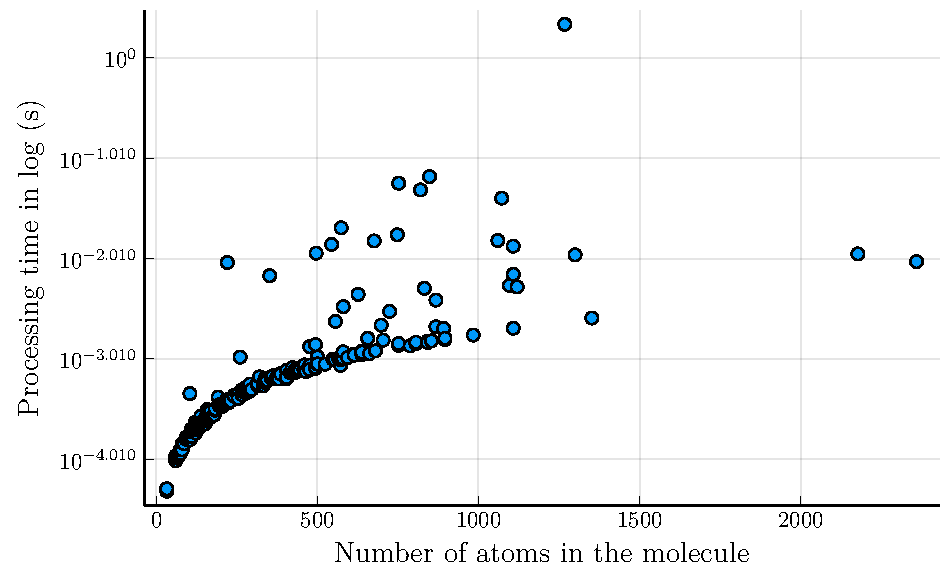
\includegraphics[scale=0.55]{figures/timeMatrix.pdf} & 
			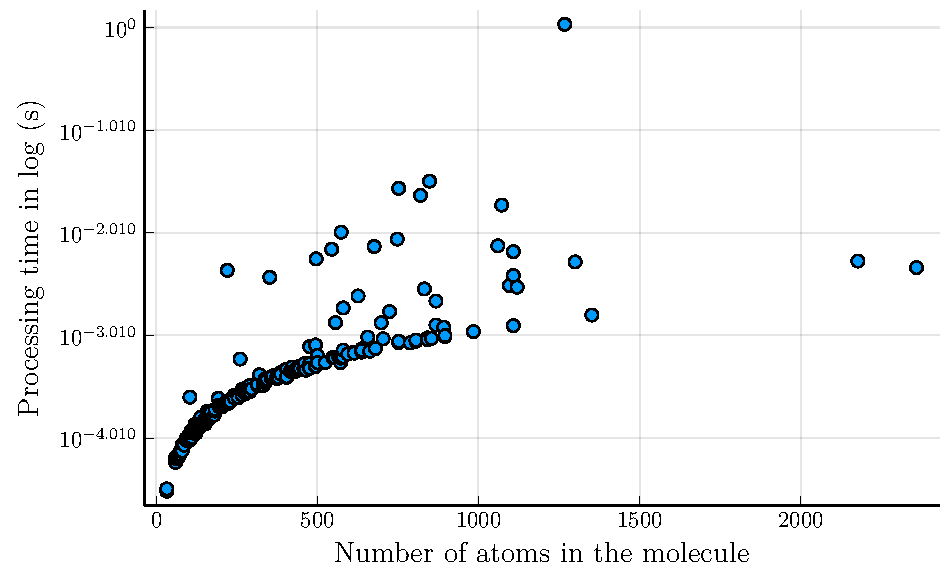
\includegraphics[scale=0.55]{figures/timeQuaternion.pdf} \\
			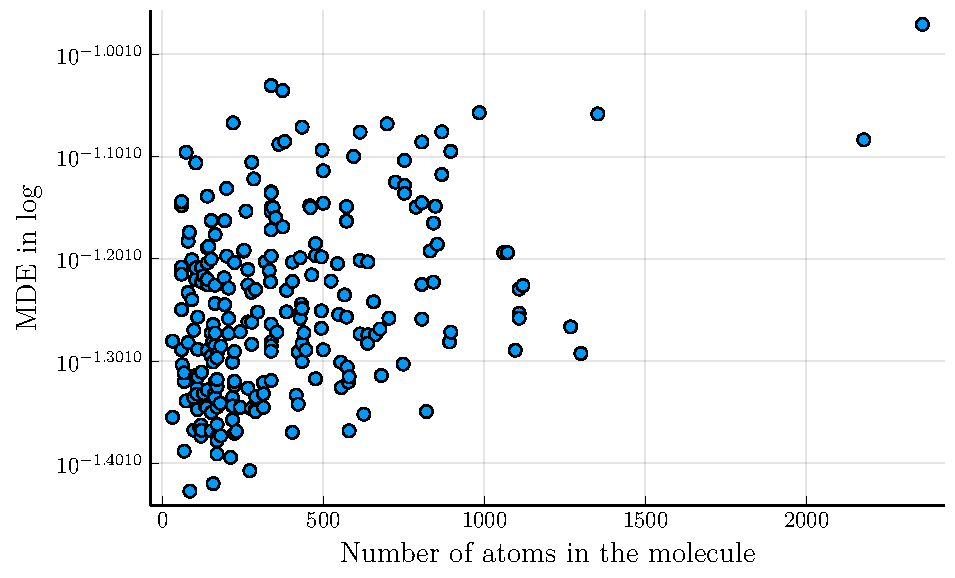
\includegraphics[scale=0.55]{figures/MDEMatrix.pdf} &
			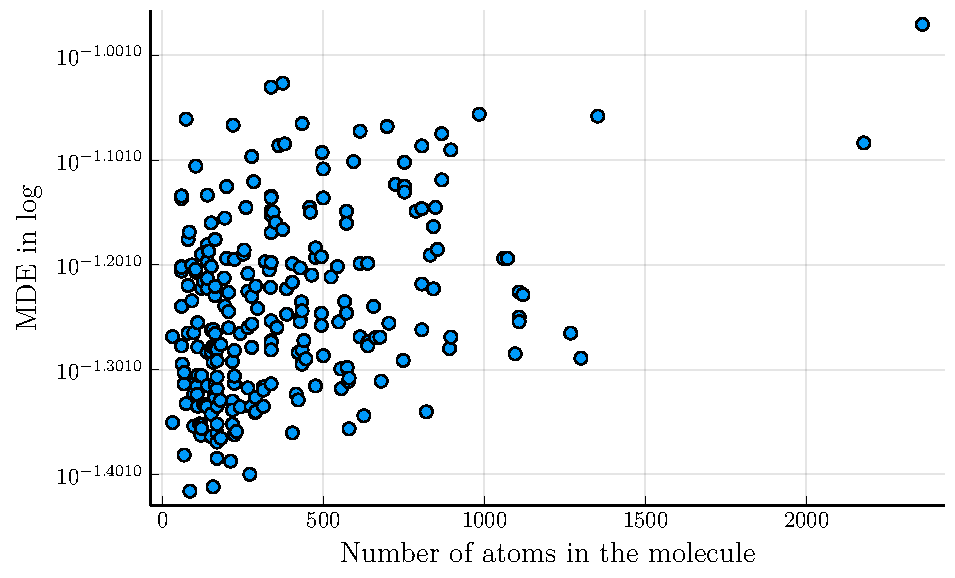
\includegraphics[scale=0.55]{figures/MDEQuaternion.pdf} \\
			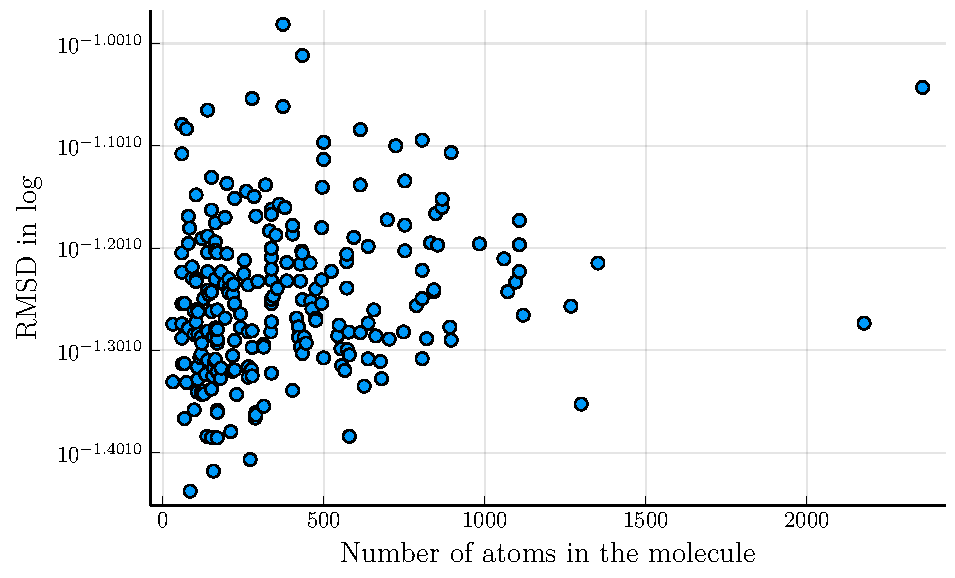
\includegraphics[scale=0.55]{figures/RMSD.pdf} &
			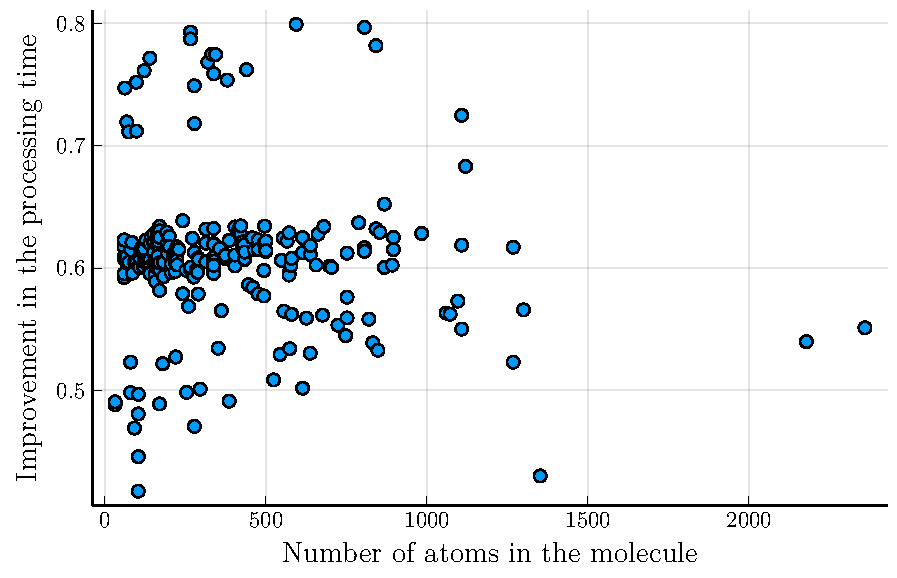
\includegraphics[scale=0.55]{figures/improv.pdf} \\
			\multicolumn{2}{c}{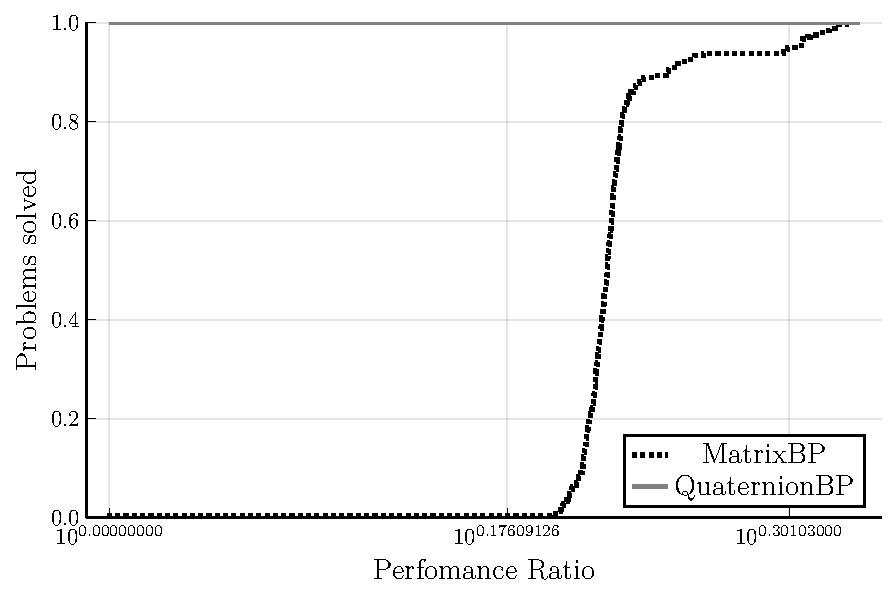
\includegraphics[scale=0.55]{figures/perfomance_profile.pdf}}\\
		\end{tabular}
		\label{fig:mean}
	\end{figure}
	
	\newpage
	\subsection{BP-All}
	\begin{figure}[H]
		\begin{tabular}{cc}
			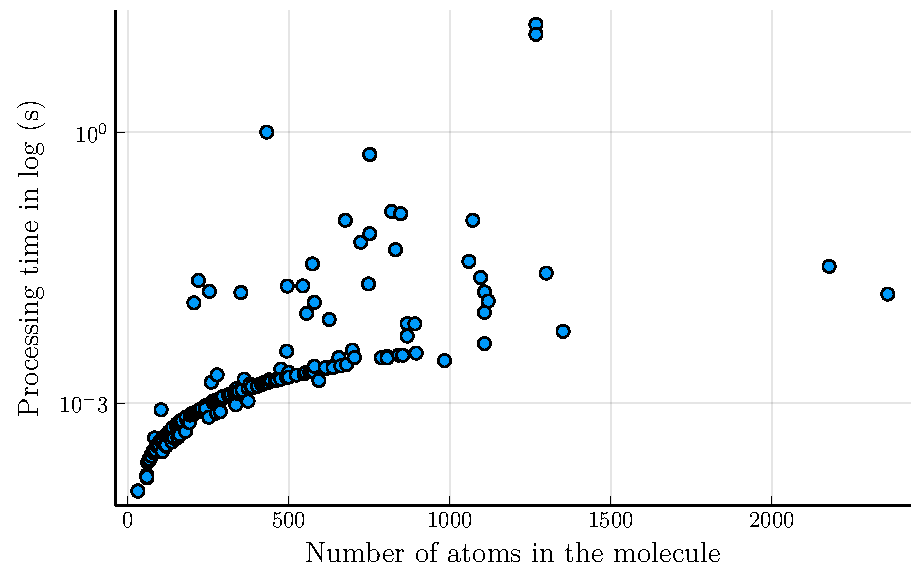
\includegraphics[scale=0.55]{figures/timeMatrixAll.pdf} & 
			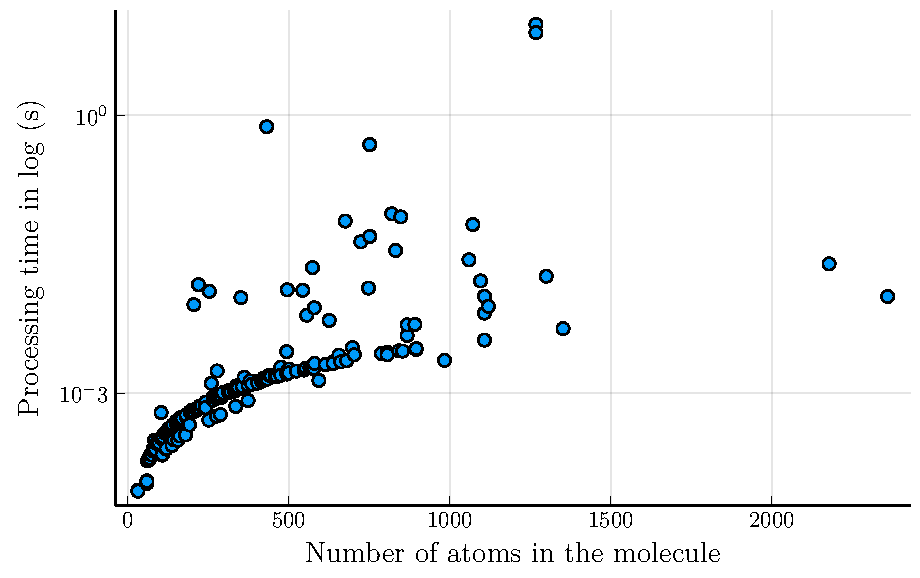
\includegraphics[scale=0.55]{figures/timeQuaternionAll.pdf} \\
			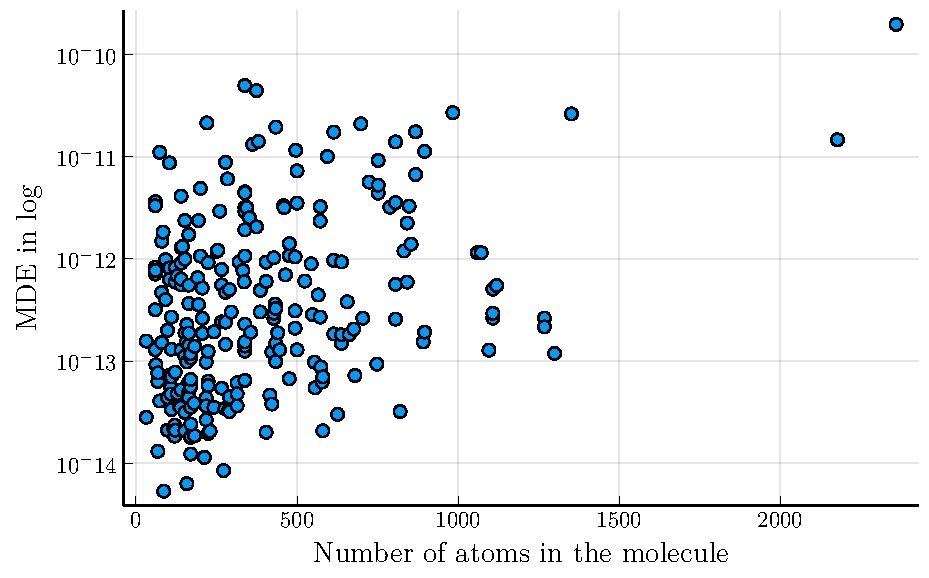
\includegraphics[scale=0.55]{figures/MDEMatrixAll.pdf} &
			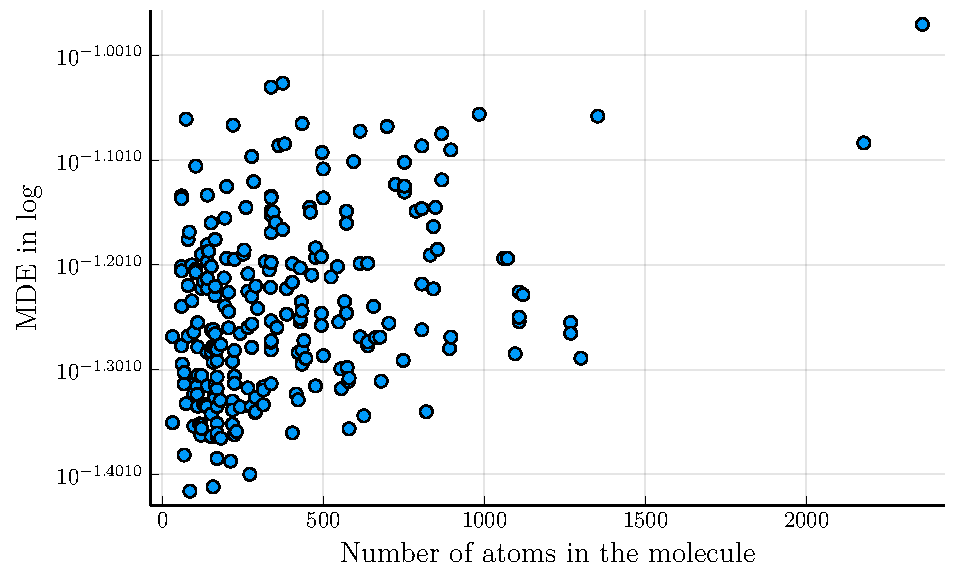
\includegraphics[scale=0.55]{figures/MDEQuaternionAll.pdf} \\
			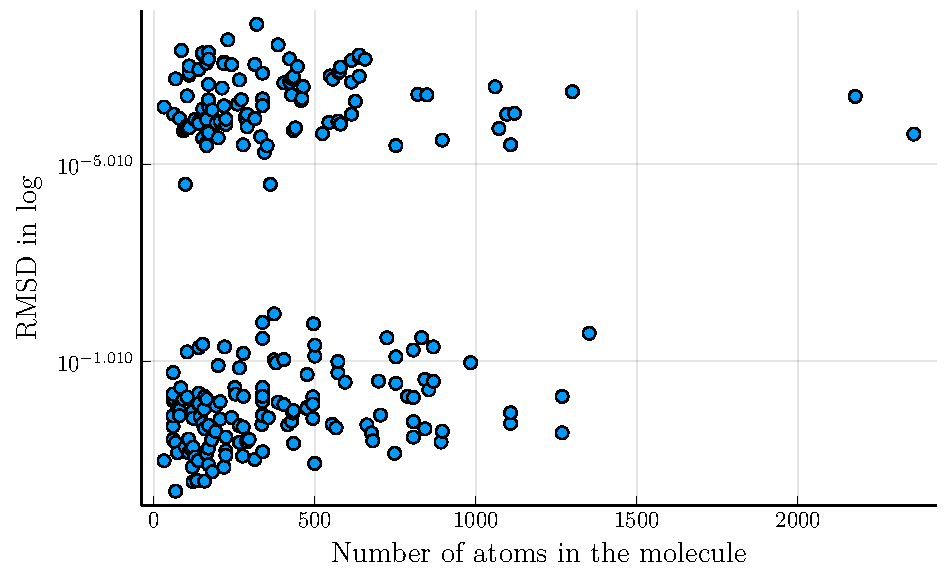
\includegraphics[scale=0.55]{figures/RMSDMatrixAll.pdf} &
			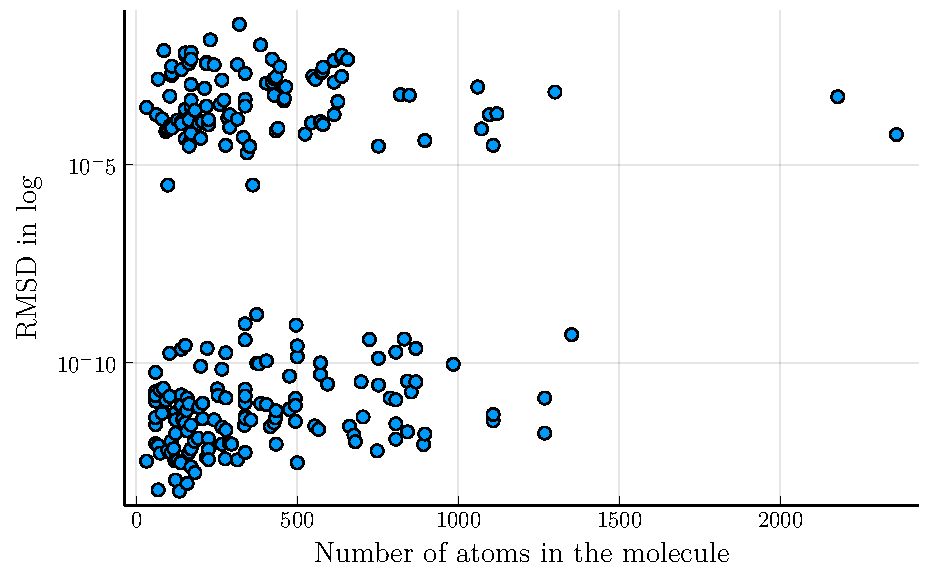
\includegraphics[scale=0.55]{figures/RMSDQuaternionAll.pdf} \\
			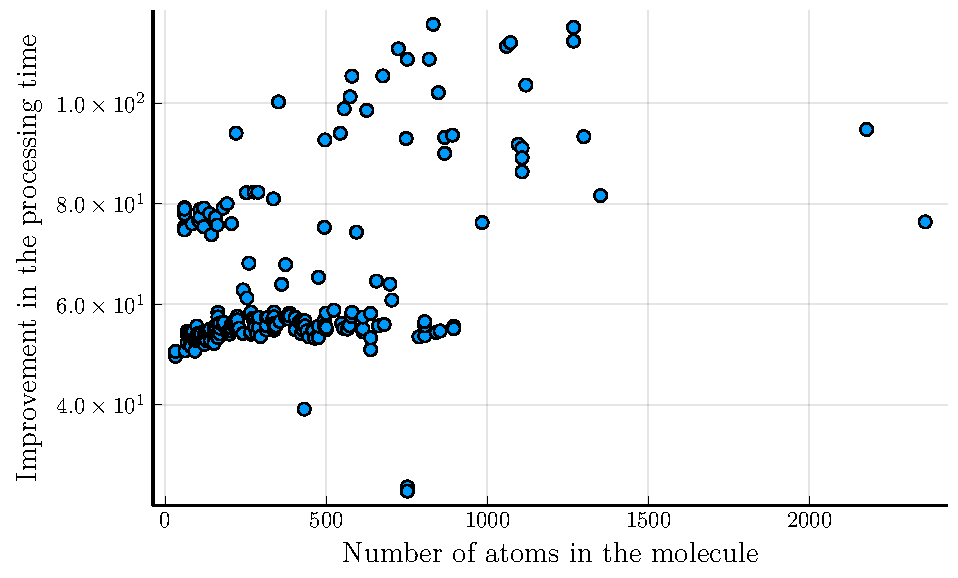
\includegraphics[scale=0.55]{figures/improvAll.pdf}& 
			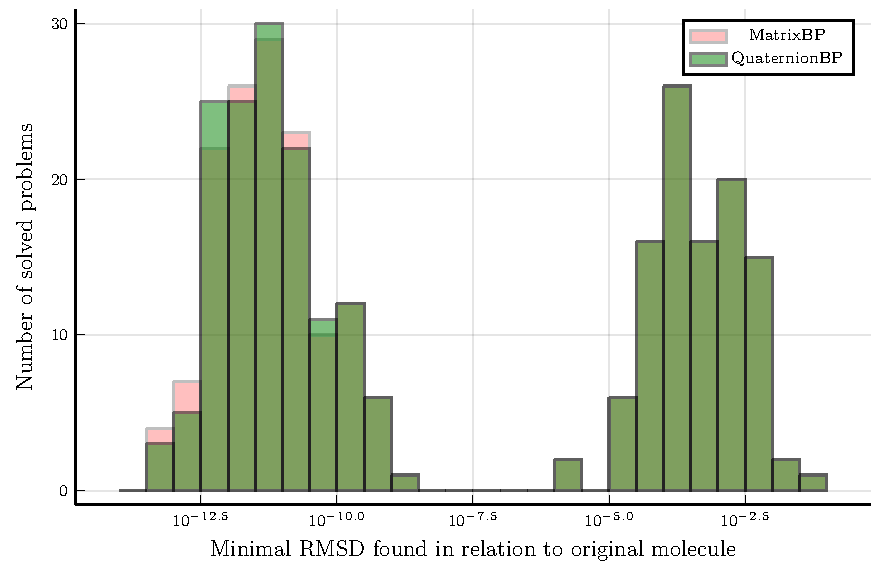
\includegraphics[scale=0.55]{figures/histogramRMSD.pdf} \\
		\end{tabular}
		\label{fig:mean}
	\end{figure}

\end{document}	